% !TeX spellcheck = en_GB
%\documentclass[11pt,DIV=11,a4paper,BCOR=15mm,twoside=on,bibliography=leveldown]{scrbook}
%\documentclass[11pt,DIV=11,a4paper,BCOR=15mm]{scrbook}
\documentclass[%
  11pt,
  DIV=16,
  a4paper,
  BCOR=15mm,
  twoside=on,
  bibliography=totoc,
  headings=normal,
  titlepage
%  captions=tableheading,
%  chapterprefix=true% like in standard class "report"
]{scrreprt}
%\documentclass[11pt,DIV=11,a4paper]{scrartcl}
\usepackage{ma}

\title{Modelling and Automated Retrieval of Provenance Relationships}
\author{Thomas Schneider}

\begin{document}

  \pagenumbering{roman}
  % \maketitle
  \selectlanguage{ngerman}
  % !TeX spellcheck = de_DE
\thispagestyle{plain}
\begin{titlepage}

  \begin{center}
  
    \vspace*{1cm}
    Humboldt-Universität zu Berlin \\
    Philosophische Fakultät \\
    Institut für Bibliotheks- und Informationswissenschaft
  
    \vspace*{\fill}
    {\Huge\bfseries\sffamily
      Modelling and Automated Retrieval \\[6pt]
      of Provenance Relationships
    }
    
    \vspace*{\fill}
    Masterarbeit im Rahmen des Weiterbildenden Masterstudiengangs\\
    Bibliotheks- und Informationswissenschaft im Fernstudium
    
    \vspace*{\fill}
    vorgelegt von \\
    Thomas Schneider
    
    \vspace*{\fill}
    Gutachter: \\
    Prof.\ Dr.\ Robert Jäschke \\
    Christian Rüter
    
    \vspace*{\fill}
    Erfurt, den \today
    
    \vspace*{1cm}
    
%    \copyright\ 2023\\[9ex]
  
  \end{center}
  
%%  \singlespacing
%  \small
%  \noindent Dieses Werk einschließlich seiner Teile ist \textbf{urheberrechtlich geschützt}. Jede Verwertung außerhalb der engen Grenzen des Urheberrechtgesetzes ist ohne Zustimmung des Autors unzulässig und strafbar. Das gilt insbesondere für Vervielfältigungen, Übersetzungen, Mikroverfilmungen sowie die Einspeicherung und Verarbeitung in elektronischen Systemen.

\end{titlepage}
%  \setcounter{tocdepth}{2}
  \selectlanguage{UKenglish}
  \tableofcontents

%  \clearpage
%  % !TeX spellcheck = en_GB
% =================================================================
\chapter*{Sketchbook}

% -------------------------------------------------------------------
\section*{``Storyline''}

\begin{tikzpicture}[
  >=Latex,
  every node/.style={draw=none,fill=none,thick,inner sep=1.5mm},
  every edge/.style={draw=black,thick}  
]
  \node                                 (queries)         {Prototype queries};
  \node [below=10mm of queries]         (datasources)     {\tikztab[c]{Requirement analysis:\\[-1pt]Analysis of available data sources\\[-1pt]Analysis of possible queries}};
  \node [below=10mm of datasources]     (modelling)       {Modelling};
  \node [below=10mm of modelling]       (dataintegration) {Data integration};
  \node [below=10mm of dataintegration] (method)          {Method};
  
  \path[->]
    (queries)         edge (datasources)
    (datasources)     edge (modelling)
    (modelling)       edge (dataintegration)
    (dataintegration) edge (method)
  ;
  
\end{tikzpicture}

\begin{itemize}
  \item 
    Modelling depends on requirement analysis: why is it appropriate to use graphs rather than ``fully-fledged'' database theory?
  \item
    OTOH, the early specification of prototype queries will necessarily remain vague and extensional
    as long as we don't have an abstract model!
  \item
    perhaps use ``lightweight'' def. of a conjunctive query?
\end{itemize}


%
  \clearpage
  \pagestyle{headings}
  \pagenumbering{arabic}
  % !TeX spellcheck = en_GB
% =================================================================
\chapter{Introduction}
\label{chap:intro}

% -----------------------------------------------------------------
\section{Setting}
\label{sec:setting}

In research on the historical holdings of university and research libraries,
the origins of book copies\todo{really restrict to books?} are of central importance.
The origin of an item is also called its \emph{provenance} 
and comprises the people or corporations that owned this item over time.
Particularly interesting provenances are those related to the change of
owners when book copies are passed on or distributed \autocite[p.\,2]{Hakelberg2016}.
Provenances can be reconstructed by marks of ownership
such as stamps, bookplates (ex libris), or handwritten signatures:
with the help of these features, it is possible to retrace
the ``history'' of a book copy
or the extent of library holdings that have been scattered in the meantime \autocite[p.\,2]{Hakelberg2016}.

In order to enable provenance research,
libraries index the provenances of their historical holdings
and make them available to users via their catalogues.
A provenance entry refers to a person or corporation
and to a feature that indicates ownership.
In order for owners to be identified unequivocally,
they are often given via a reference to authority files such as the
Integrated Authority File (GND) of the German National Library.%
\footnote{%
  \url{https://www.dnb.de/EN/Professionell/Standardisierung/GND/gnd.html}%
}
The indexed provenance data makes it possible, for example,
to query and reconstruct the books owned or held by a single person or corporation,
to query the whereabouts of relevant copies,
or to retrace the distribution of all indexed copies of a work.

In the digital age, provenance entries are recorded in electronic catalogues.
German university and research libraries typically do not 
maintain their own individual catalogue; rather they are provided with a central
catalogue by the library network in which they participate.%
\footnote{%
  There are six library networks \emph{(Bibliotheksverbünde)} for scientific libraries
  in Germany: \url{https://de.wikipedia.org/wiki/Bibliotheksverbund\#Deutschland}%
}
These central catalogues are equipped with an underlying database
and standardised data formats for internal representation and data export.
For example, the networks GBV and SWB maintain and use the common catalogue (database)
\emph{K10plus},%
\footnote{\url{https://www.bszgbv.de/services/k10plus/}}
which internally uses the data format PICA%
\footnote{\url{https://format.gbv.de/pica}}
and allows for exports in the data formats
MARC 21, MAB2, and Pica+.%
\footnote{\url{https://wiki.k10plus.de/display/K10PLUS/Exportformate}}
%  \footnote{\url{https://de.wikipedia.org/wiki/Machine-Readable_Cataloging}}%
%  \footnote{\url{https://www.dnb.de/DE/Professionell/Metadatendienste/Exportformate/MARC21/marc21_node.html}}
Despite the use of a uniform data format,
there are several possibilities to record provenance entries.
As Hakelberg \autocite*[Chapter~4]{Hakelberg2016} explains,
libraries even within the same network often use diverse representations
for the same type of provenance entry, and the differences are considerable:
for example, some GBV libraries record their provenance entries
in data fields on the bibliographic level,
while others use the level on the exemplar level.
These deviations lead to large differences in the presentation
of the holdings in the online catalogue,
which hinders the retrieval of relevant copies and historical holdings.

Data about persons and corporations are recorded
in Germany- or worldwide authority files and further databases,
such as the previously mentioned GND,
the \emph{WorldCat},%
\footnote{\url{https://www.worldcat.org/identities/}}
databases of projects such as ISNI%
\footnote{\url{https://isni.org/}}
and VIAF%
\footnote{\url{https://viaf.org/}}
or in Wikidata.%
\footnote{\url{https://www.wikidata.org/wiki/Wikidata:Main_Page}}
These data sources usually support standardized data formats for data export,
such as MARC~21 and RDF via several interfaces in the case of GND.
Data about a person contain, among others, the name and alternative name forms
(which can be manifold in the case of, e.g., scholars of previous centuries),
places of birth, death, and work,
as well as relationships to corporations and other persons
(e.g., coauthors and students).
The extent of a dataset of the same person can differ between data sources,
which is witnessed, for example, by the entries on the scholar
Georg Joachim Rheticus in ISNI, VIAF, WorldCat, GND, and Wikidata.%
\footnote{%
  This can be verified by following,
  at the end of the Wikipedia page on Rheticus 
  in the table „Authority Control“ \url{https://en.wikipedia.org/wiki/Georg_Joachim_Rheticus\#External_links}\,,
  the links to ISNI, VIAF, WorldCat und GND,
  and inspecting the Wikidata data set
  \url{https://www.wikidata.org/wiki/Q93588}\,.
}
Hence, the state of data on persons and corporation is heterogeneous as well,
and depending on the concrete individual, it may be necessary
to consult several data sources and combine the obtained data.

Given this diversity and heterogeneity of the existing data sources,
it is currently difficult to impossible to retrieve provenance relationships
that are not restricted to bibliographic items and their owners
but which also involve various relationships between works, copies, and (multiple) owners.
For example, one could be interested in answers to the following queries.
%
\begin{enumerate}
  \item[\exaquery{1}]
    Who read work $W$, in which manifestation and in which year?
  \item[\exaquery{2}]
    Which copies of work $W$ were passed from one of its owners to a collaborator (or a student)?
  \item[\exaquery{3}]
    What are the relationships between the recipients of work $W$
    (or of manifestation $M$ of $W$ or of copy $C$ of $W$, respectively)?
\end{enumerate}
%
Query~\exaquery{1} addresses works as well as their manifestations
(e.g., editions of the same work in various languages).
An answer to this query would allow it to trace the reception
of the same work over several eras. For example, Duchess Luise Dorothea of Saxe-Gotha-Altenburg
read French editions of English works.\todo{give more concrete example}\footnote{Dietrich Hakelberg, personal communication}
%
Queries~\exaquery{2} and~\exaquery{3}
aim at highlighting the network
that spans between the recipients of a work.
For example, one of the two copies of Nicolaus Copernicus's
main work \emph{De revolutionibus orbium coelestium} \autocite{Kopernikus1543}
that are now held by the Gotha Research Library of the University of Erfurt
have been owned, or at least read, by several scholars
from the circle around the author,
some of which were in the teacher-student relationship;
this can be verified using the accounts of Gingerich~\autocite[p.\,69]{Gingerich2002}
and Salatowsky and Lotze~\autocite[p.\,142]{Salatowsky2015}
or looking up the entry in the electronic catalogue of the library.%
\footnote{\url{https://opac.uni-erfurt.de/LNG=EN/DB=1/XMLPRS=N/PPN?PPN=567506266}, field ``Provenance(s)''}
%
An important difference between \exaquery{2} and~\exaquery{3} is the following.
While \exaquery{2} fixes a relationship between two persons (``collaborator'' or ``student'')
and asks for works in whose context this relation occurs,
\exaquery{3} does not fix a particular relationship but asks for the entire context of
the work or a manifestation or copy thereof.

In order to answer queries such as \exaquery{1}--\exaquery{3},
it does not suffice to consult a single data source such as
a catalogue, authority file, or knowledge base.
Instead, it is necessary to consult several data sources
and combine the information found. This process is highly laborious,
given not just the number of data sources but also their diverse
data formats. Therefore, automated support is essential.
This is one of the reasons for Hakelberg
to raise the following question \autocite[p.\,46, translated from German]{Hakelberg2016}:
``How can historical provenance relationships be formulated and represented
in a machine-readable way?''

In order to implement suitable tools,
it is necessary to analyse available data sources, data models, and data integration techniques,
to develop an abstract model of data sources and possible queries,
and to devise a method for obtaining answers in this abstract framework.

% -----------------------------------------------------------------
\section{Aim and Research Question(s)}
\label{sec:research_questions}

\todo[inline]{TODO: import from \emph{Exposé}}

We want to develop a method for answering provenance queries that refer to bibliographic entities, people, and corporations
as well as the relationships between those. This method should consult standard data sources such as 
library catalogues, authority files, and knowledge bases. The method should furthermore be implementable as a software tool
that supports the user in formulating their queries, answering them, and exploring the data that supports the query answers.
In the long term, we envisage that such a tool will support provenance research
by prospectively retrieving potentially interesting constellations.

% -----------------------------------------------------------------
\section{Outline}
\label{sec:outline}

\begin{itemize}
  \item
    review of related work: Chapter~\ref{chap:rel_work}
  \item
    discussion of prototype queries: Chapter~\ref{chap:prototype_queries}
  \item
    analysis of available data sources and techniques: Chapter~\ref{chap:analysis}
  \item
    generic model of data sources, queries, and answers: Chapter~\ref{chap:modelling}
  \item
    method for answering queries: Chapter~\ref{chap:retrieval}
  \item
    conclusion and outlook: Chapter~\ref{chap:conclusion}
\end{itemize}



  % !TeX spellcheck = en_GB
% =================================================================
\chapter{Context}
\label{chap:rel_work}
\label{chap:context}

This thesis aims at providing support for provenance research, which is part of historical research.
As we have seen in Chapter~\ref{chap:intro}, networks that represent
people and their relationships play a central role.
Therefore, we begin our exploration of the scientific context of our work
with the topic of historical (social) network analysis.
We will collect insights from a recent research project
aimed at providing a research infrastructure for historical network analysis
and apply them to our research questions.

It has also become clear in Chapter~\ref{chap:intro} that the relevant data is distributed 
over a multitude of heterogeneous data sources.
Therefore we will review the literature on linked data, data integration,
and data provenance.

Furthermore/finally \dots

\todo[defer,inline]{\enquote{announce} knowledge graphs, state of provenance indexing, further research}

\todo[quick,inline]{end each par containing a summary to related work with \enquote{[cf.\ $<$source$>$]}}

% -------------------------------------------------------------------
\section{Network Analysis and the SoNAR Project}
\label{sec:HNA+SoNAR}


% - - - - - - - - - - - - - - - 
\subsection{Network Analysis}

According to Jansen \autocite*{Jansen2003},
the notion of a \emph{network} is a central tool for the analysis
of modern societies in sociology, political science, and economics.
In these disciplines, networks of political actors, companies, or researchers,
among many others, are the subject of study.
Additionally, networks play an important role
in organisational psychology, biology, and web science \autocite{WikiSNAGerman,WikiNetworkAnalysis}.
%As we will see in the remainder of this section,
%networks and their analysis are essential tools
%in the context of the approach that we are going to develop.
%Therefore, the next 
The following
paragraph briefly summarises the main constituents of network analysis
as described by Jansen \autocite*{Jansen2003}.

\emph{Network analysis}
defines networks and provides a statistical toolset for describing and analysing them.
A network is a graph, which consists of nodes and edges.
Nodes represent actors, events or objects (e.g., people, companies, institutions, countries),
and edges represent relations between those (in the case of social networks, e.g.,
friendship, collaboration, or family relationships).
Networks are defined via certain modelling decisions
such as the commitment to a set of actors and relations that are of relevance,
or the decision whether relations are directed or undirected
and whether they are dichotomous (an edge is present or not)
or weighted by values representing frequencies or extent.
The tools provided by network analysis include
various metrics that apply to single nodes, pairs of nodes, paths in the network,
or the whole network; those often come in several variants.
Examples are connectivity, in-/outdegree, density,
size, cohesion, multiplexity, reachability, and path distance.
Since a graph can conveniently be represented by its adjacency matrix,
methods from matrix algebra are part of the toolset.

In applications where social structures are the object of study,
the term \emph{\gls{SNA}} is used,
and it predominantly refers to the \emph{method} of investigating
social interactions \autocite{Otte2002}.

In the context of historical research,
the notion of \emph{\gls{HNA}}
has emerged recently; it focusses on the reconstruction of
historical networks \autocite{Menzel2020}.
A distinguishing feature of \gls{HNA} is its retrospective view,
i.e., it is used to analyse historical data extracted
from available sources \autocite{Fangerau2022}.
Menzel et al.\ \autocite*{Menzel2020} name
\enquote{a lack of awareness with regard to the availability of suitable research data}
as a limiting factor of \gls{HNA};
in particular, a large amount of data is distributed over heterogeneous data sources.

% - - - - - - - - - - - - - - - 
\subsection{SoNAR (IDH)}

The project \enquote{SoNAR (IDH),
Interfaces to Data for Historical Social Network Analysis
and Research} \autocite{Bludau2020,Menzel2020,SoNAR},
%\glsunset{SoNAR}%
which was funded by the German Research Foundation (DFG)
from 2019 to 2021,
developed approaches to building 
\enquote{an advanced research technology environment
supporting Historical Network Analysis and related research} \autocite{SoNAR}.
In the long-term vision, that environment is expected to
integrate data from a variety of existing repositories,
thus providing researchers with an extensive,
standardised, and interregional infrastructure for answering research questions
using methods from \gls{HNA}.
According to the project proposal and the final reports \autocite{SoNARreports},
the project participants undertook
a systematic analysis of processing and managing the source data
for the purposes of \gls{HNA},
designed a model of a structured data analysis for \gls{HNA} based on \gls{SNA} methods,
developed visualization approaches and interfaces,
evaluated all components for a scientific usage,
and developed a concept for implementation and operation.

One of the project's four work packages (WPs)
addresses the development of the research technology environment
and its evaluation against real research questions.
In the following paragraphs,
we summarise the insights described in the final report on this WP \autocite{Fangerau2022}
that are relevant for the research goals of this thesis.

The report emphasises relationships and their evolution over time
as central aspects of historical research and acknowledges the increased 
importance of methods of \gls{HNA}. In this context, the authors note that visualisation plays an important role
as a means for restructuring information and thus contributes to the progression of knowledge.
They also address the \emph{hermeneutic circle} \autocite{Malpas2015}
as a general approach to answering historical research questions:
this term refers to an iterative, circular work process
where the initial question guides the work with the source material
and is, in turn, readjusted based on the answers obtained.

In order to evaluate the research technology,
the project participants developed two research scenarios
with several research questions.
The report names four concrete questions that were considered central.
The nature of these questions is very general and \enquote{global}
in the sense that they refer to a large part of a network:
for example, they ask for the point in time when a scientific area became a separate discipline,
or for the role of academic and familial links in the course of a given scientist's career.

In this context, the report distinguishes two approaches to developing research questions
in \gls{HNA}. One of these is the explorative approach,
where suitable questions are developed based on the available data.
According to the authors, this approach includes serendipity,
i.e., the hope that an inspection of the data helps identify unexpected
phenomena that contribute to the shaping of the research question.

The report uses the term \emph{data source} for original documents, media, and artefacts
from which \enquote{network-compatible} (i.e., essentially relational) data can be obtained;
data sources can be identified via \emph{repositories} of various kinds,
including library catalogues, archive portals, databases, and more.
The report highlights the advantages of using data from authority files
such as the \gls{GND}, which are standardised,
subject to quality control, and essential for disambiguating personal names.
Moreover, authority files are freely accessible and provide information
on the provenance of their data.
%According to the authors,
%\enquote{the use of authority data from \gls{GND} in SoNAR is a unique feature
%of the research technology environment and has, in principle, proved its worth}.

Concerning the repositories used,
the authors report the general problem of missing or erroneous data,
which leads to distorted answers to the questions, and which was not solved
systematically in the project. In particular, the \gls{GND} is focused on German library holdings
and thus contains a disproportionately high amount of German-speaking persons.
The data is biased towards people who have published at all,
towards elite research, towards men (in particular among authors before the 1950s),
and against certain disciplines, such as economy.
The authors conclude that these restrictions significantly affect the answers to
historical research questions. As possible remedies, they include 
further repositories, such as 
the \gls{ZDB},
the \gls{DNB},
the \gls{KPE},
and, tentatively, other authority files (in particular, Wikidata and \gls{VIAF});
we will get back to these in Section~\ref{sec:data_sources}.
However, the evaluation showed that even the sum of these repositories
does not provide enough data for a differentiated temporal
analysis; in particular, biographical data of the authors 
dominate, but those cover long time spans and do not provide sufficient evidence
for or against dynamic relationships such as teacher-student relationships.

%\enquote{allow a temporal differentiation over longer periods of time} (translated).

Concerning the selection of data, the report distinguishes between
direct and indirect information on relationships.
For example, if one is looking for support for the hypothesis of a social relationship
between two persons $A$ and $B$, then a family relationship between $A$ and $B$ explicit in the data
supports the hypothesis directly, while matching biographical dates for $A$ and $B$
are an indirect indicator. In the latter case, the relationship
explicit in the data (matching biographical dates) acts as \emph{substitute information}
(\enquote{Stellvertreterinformation}) for the relationship under consideration.
The authors also address a special kind of indirect relationship,
called intellectual, which mostly involves a third person
or event, such as the co-citation of $A$'s and $B$'s texts by someone else.

A main constituent of the report is a catalogue of requirements
to \gls{HNA} and the research technology. This catalogue consists of 61
requirements that reflect the specific needs of researchers.
The following of these requirements are relevant for our purposes
(descriptions translated from the original German text and slightly rephrased and/or shortened):
%
\begin{description}
  \item[R003]
    Researcher wants all information on relationships contained in the metadata of the resources
    to be shown as derived social relationships in the data model.
  \item[R004]
    Researcher wants all information on non-social
    relationships (see above) to be distinguished from direct social relationships.
  \item[R005]
    Researcher wants to connect non-social and non-explicit social relationships
    with further conditions (e.g., overlapping lifespans).
  \item[R006]
    Researcher wants to group people with comparable attributes (e.g., overlapping lifespans).
  \item[R016]
    Researcher wants a list of people connected to a given person.
  \item[R017]
    Researcher wants a list of corporate bodies connected to a given person.
  \item[R018]
    Researcher wants a list of people connected to a given person via some corporate body.
  \item[R029]
    Researcher wants, given a node, a description of the \enquote{potentially available attributes}
    and the provenance of the data.
  \item[R030]
    [dito, but with edges instead of nodes]
  \item[R043]
    [Researcher wants] a filter on attributes, e.g. biographical data, in order to
    restrict relationships to adulthood.
  \item[R061]
    Researcher wants to know which kinds of relationships are contained in the dataset.
\end{description}

% - - - - - - - - - - - - - - - 
\subsection{Graph Technologies for the Analysis of HNAs Using Heterogeneous Data Sources}

In the paper of the same name, \textcite{Menzel2020} report on
work in the \gls{SoNAR} project concerning the 
\enquote{creation and operation of research infrastructure
for [\gls{HNA}] based on heterogeneous data sources from cultural heritage institutions}.
In particular, the authors present insights on modelling and transformation
of heterogeneous data sources and on the design of visualisation for historical networks.
We summarise their insights on data selection and processing.

In the described approach, the authors integrate data from 6 heterogeneous repositories
into a large uniform graph that is stored in a graph database
and managed by the highly performant graph database management system Neo4j \autocite{Neo4j}.
The original repositories comprise an authority file \gls{GND},
federated library catalogues (\gls{DNB}, \gls{ZDB}, \gls{KPE}), %\autocite{DNBCatalogue,ZDB,KPE}),
and full texts (ZEFYS, Exile Press \autocite{ZEFYS,ExilePress});
altogether they contain some 30 million records.
The data model is restricted to 9 entity types (e.g., \term{Resource} or \term{PersonName})
and 9 very generic relation types (e.g., \term{RelationToPersonName}, \term{RelationToTopicTerm}).
There is also a distinction between explicit and implicit relations:
the former are present in the data, and the latter have to be inferred automatically via
certain \enquote{guidelines} and marked as such.

Since some of the above data sources include full texts,
it is necessary to link names of people, corporate bodies, or geographical entities
to entities in authority files. The use of the underlying technique,
\emph{named entity linking}, is discussed further by \textcite{Menzel2021}
in the context of \gls{SoNAR},
and by \textcite{Meiners2022} independently of \gls{SoNAR}.

Among the challenges associated specifically with processing data,
\textcite{Menzel2020} name
the sheer size of the combined graph, which causes performance issues,
and the fact that the normalisation led to errors and inconsistencies.
More generic challenges include the integration of domain knowledge
and the adaptation of a more performant graph database engine (GraphDB),
which requires extensive remodelling.

\todo[think,inline]{Some more comments on NEL and choice of data sources from \autocite{Menzel2021, Meiners2022}? see Exposé}

% - - - - - - - - - - - - - - - 
\subsection{Insights Relevant for This Thesis}
\label{sec:insights_from_SoNAR}

We now put the insights from the \gls{SoNAR} project described in the previous two subections
into relation with the research goals pursued in this thesis.
First, the analysis of historical networks is a broad concept, and \gls{SoNAR} supports a setting
that is much more general than just provenance research.
Thus, the setting that we want to support in this thesis is a specific section of \gls{HNA} and subsumed 
by the \gls{SoNAR} setting.

The central role of relationships and of temporal aspects in historical research
have to be reflected in the model and method that we are going to develop.
Furthermore, the hermeneutic approach to historical research
and the explorative approach to answering general research questions 
need to be supported by our method. In fact, the repeated exploration of data
is exactly what we hope to support by enabling researchers to ask specific
queries over a combination of data sources and use the answers to obtain
\enquote{local} views of the whole network and thus inform the next steps in their research process.

\emph{Locality} is an important feature that distinguishes our approach from the \gls{SoNAR} setting:
The exemplary research questions from the \gls{SoNAR} report appear to be rather global
in the sense that they focus on wider areas in the network and that their analysis requires
\enquote{global} techniques such as graph metrics and statistical methods.
In contrast, we aim at answering more local queries
that are part of a larger research question and which 
focus on a single item/actor and its neighbourhood in the network
(e.g., owners of a book or students of a scholar, see the exemplary questions
in Section~\ref{sec:background}). Answering such queries
requires the retrieval of certain \enquote{candidates} from that neighbourhood
which provide the necessary evidence and which then can be used
to inform another iteration within the explorative approach.
In the light of these considerations, 
we should not adopt the a-priori restriction
to a fixed set of entity types or (generic) relation types;
instead, it should be to use arbitrary concepts and relations
from the data sources in queries and answers.
Hence, we will focus on the described local perspective
and leave the accommodation of global techniques for future work.
In a similar spirit, we will not study visualisation;
however, our envisaged tool can be used \emph{along with} visualisation tools
and provide entry points to a large network.

The construction of a uniform data source \emph{(graph)} that integrates all the available data
from the heterogeneous repositories appears to be an integral part of \gls{SoNAR},
according to \citeauthor*{Menzel2020}'s \autocite*{Menzel2020} discussion.
The obvious advantages include the interaction with a single database,
the use of a single data model, autonomous hosting
independently of the single repositories, and thus full control over the data.
Furthermore, inconsistencies
between the repositories can be resolved a-priori (at creation time),
and the created database is independent on possible changes in the data models of the repositories.
However, the static nature of the uniform database also has disadvantages:
a data model has to be fixed upfront, and ultimately needs to be adapted when
the models of the repositories change or new repositories are added;
regular updates are necessary when the contents of the repositories changes;
finally, as we have learnt above,
a large graph database uses a large amount of memory and requires a highly performant
database system.

As a result of this discussion,
we want our approach to exploit the benefits of a dynamic solution.
More precisely, while our abstract model will centre around a single data source (graph)
that represents the combination of the distributed repositories,
our method will abstain from constructing that graph explicitly and, instead,
answer queries \enquote{in place} over the original repositories.
This way, our approach will not depend on hosting capacities,
and it will always have direct access to the current content of the repositories.
On the downside, our approach will depend on external web services provided by the repositories,
and it will be sensitive to changes in their data models.
Our dynamic approach also requires that inconsistencies are resolved
a posteriori, i.e., every time a query answer is retrieved.
As a final advantage, the dynamic approach is flexible
in the sense that it can be applied to a static integrated data source as well,
thus benefiting from the advantages of the static approach.

A feature that we miss in the reports and publications of \gls{SoNAR} is a rigorous definition of admissible queries
that specifies exactly which queries are in the scope and which are not.
We aim at providing such a rigorous definition for our setting
which, at the same time, should be as general as possible. We consider this rigorous definition
a main feature of our approach.

Data sources in the sense used in the \gls{SoNAR} project report,
i.e., original documents, media, and further artefacts
are not part of our setting, as we do not consider the part of the research process
that consults those data sources. Our work focuses on the level of
what the \gls{SoNAR} authors refer to as repositories,
and we will relate our choice of repositories in Section~\ref{sec:data_sources}
to \citeauthor*{Menzel2020}'s \autocite*{Menzel2020} selection.
In this thesis, we continue to use the term \enquote{data source} for what
\gls{SoNAR} refers to as a repository,
and we speak of \emph{original data sources} to refer to original documents etc.

In order to allow researchers to refer to the original data sources,
it becomes clear that \emph{data provenance} plays a crucial role:
the answer to a specific query in our approach needs to refer to
the original data sources that provide evidence for the information contained in that answer.
This reference can point to original documents (\gls{SoNAR}: data sources),
and/or to data sets in repositories. For a more detailed discussion of data provenance,
see Section~\ref{sec:data_provenance}.

The observed relevance of indirect or substitute information in the context of \gls{SoNAR} 
seems important to keep in mind for our work as well: 
It has to be noted that not all information that one might be looking for is recorded
in the data. For example, there is no record of who \emph{read} a book,
and ownership has to be used as a substitute for readership although evidence
of ownership is only a necessary condition for readership and not a sufficient one---%
although one might argue that, in the case of, say, a scientist, ownership is very likely
to indicate readership.
Therefore, answers to questions
about readership retrieved on the grounds of recorded ownership require further interpretation and investigation
by the researcher who asked the question in the first place.
The example from the \gls{SoNAR} report that uses \enquote{having the same biographical dates}
as a substitute for a social relationship is very similar, but in addition
the fact that two persons have the same biographical dates is not a relationship that is
given explicitly in the data but requires a certain amount of reasoning on several attributes of the entries
for the two persons.
This general observation has to be taken into account by our approach.

Finally, the insights on advantages and disadvantages of the repositories used in \gls{SoNAR}
will affect our discussion of data sources in Section~\ref{sec:data_sources}.

% - - - - - - - - - - - - - - - 
\subsection{Further Initiatives Providing Research Infrastructures}

\textcite{Menzel2020} mention several projects that connect
decentralised and heterogeneous bibliographic data sources
and/or extract historical networks within the social sciences and humanities.
We briefly summarise some of these projects.

DARIAH-DE \autocite{DariahDE} is an association that develops
a digital research infrastructure for the arts and humanities
following the example of large digital research infrastructures for the natural sciences.
It comprises of 16 partner institutions from the academic sector
and is part of the European network DARIAH-EU \autocite{DariahEU}.
DARIAH-DE's services for research include
the development and hosting of services for data analysis and visualisation
\autocite{WikiDariahDE}.

Culturegraph \autocite{Vorndran2018,Culturegraph} is a service offered by the
\gls{DNB} which aggregates bibliographic data 
from library networks in German-speaking countries,
from the \gls{DNB} itself, and from the British Library.
According to \textcite{Vorndran2018}, Culturegraph makes over 160 million data sets
available \enquote{for data analyses, evaluation of connections and statistical analyses}.
This is achieved, among other things,
by enrichment via external data sources such as \gls{GND}
and ORCID \autocite{ORCID}, thus allowing for the identification
and disambiguation of persons.

\textcite{Menzel2020} further note \enquote{an increase in joint research projects
that are focused on the extraction of historical networks within the social sciences and the humanities.}
These projects include \emph{Six Degrees of Francis Beacon} \autocite{Warren2016,SixDegreesFB},
\emph{histoGraph} \autocite{Novak2014,histograph},
\emph{Issues with Europe} \autocite{IssuesWithEurope},
\emph{APIS} \autocite{Gruber2017,APIS},
and \emph{Gesellschaftliche Wissensproduktion in der Aufklärung} \autocite{Purschwitz2018}.
Judging from \citeauthor*{Menzel2020}'s \autocite*{Menzel2020} summary,
these projects put an emphasis on statistical methods,
visualisation, and/or exploration.

% -------------------------------------------------------------------
\section{Linked Data and Data Integration}
\label{sec:linked_data+integration}

% - - - - - - - - - - - - - - - 
\subsection{Basic Concepts}

\emph{Data Integration} refers to the problem of making a set of autonomous and heterogeneous data sources
uniformly accessible \autocite[p.6]{Doan2012}.
The current landscape of data sources includes highly structured data
represented and accessed using classical database techniques,
as well as more loosely structured data accessible via (Semantic) Web techniques.
Given this vast and diverse landscape, data integration is a complex problem,
and various techniques have been developed for this purpose.
The textbook by \textcite{Doan2012} provides a
comprehensive introduction to data integration.

In the remainder of this section,
we restrict our focus on those aspects of data integration
that are most relevant in the context of bibliographic data sources on the Web.

\emph{Linked data} \autocite{W3CLinkedData,Domingue2011} refers to data published on the World Wide Web that is structured and connected with other data.
Based on a small and uniform set of simple technologies
%---essentially HTTP URIs and the Resource Description Framework (RDF)---,
the linked data paradigm provides applications with access to \enquote{a global, unbounded dataspace} \autocite{Domingue2011}.
In the context of the Semantic Web \autocite{BernersLee2001,Marshall2003},
linked data is one of several developments aimed at making data on the Web more machine-understandable.

The main technologies underlying linked data are the following.
%
\begin{itemize}
  \item
    \emph{Uniform Resource Identifiers (URIs)} \autocite{RFC3986}:
    
    \par
    A URI is a string that is assigned to a physical or logical resource
    in order to identify that resource uniquely. URLs (Uniform Resource Locators)
    are a special case of URIs which additionally ensure that a resource
    can be located in a network and that information can be retrieved from it,
    where \enquote{network} includes, but is not restricted to, the World Wide Web (WWW).
    URIs are an integral part of RDF and the Web Ontology Language OWL (see below).
  \item
    the \emph{Hypertext Transfer Protocol (HTTP)} \autocite{HTTP}:
    
    \par
    HTTP is the fundamental protocol for data transfer and communication underlying the WWW.
  \item
    the \emph{Resource Description Framework (RDF)} \autocite{RDFPrimer}:
    
    \par
    RDF is \enquote{is a framework for expressing information about resources. Resources can be anything, including documents, people, physical objects, and abstract concepts}
    \autocite{RDFPrimer}.
    Its main ingredients are \emph{resources} and binary \emph{properties} for linking resources.
    RDF statements are \emph{triples} of the format \enquote{subject--predicate--object}
    consisting of a resource, a property, and a resource (or literal).
    Resources and properties are described using URIs.
    RDF thus provides a simple and flexible data model that is particularly useful for the publication
    and linking of data on the Web.
\end{itemize}
%
In the context of the Semantic Web, RDF and associated technologies
are important tools for the definition and use of ontologies.
For a definition of the term \enquote{ontology} in this setting, we cite \textcite{Horrocks2011}:
\enquote{A major feature of the Semantic Web is the ability to provide definitions for objects and types of objects that are accessible and manipulable from within the Semantic Web. In Computer Science, a collection of these sorts of definitions about a particular domain is called an ontology, although philosophers may (and probably will) have a different understanding of what constitutes an ontology.}
More importantly for this thesis, ontologies can be used to represent knowledge about a specific domain
or about the world in general, in an unambiguous and machine-readable way, using a formal language.
What is more, \emph{reasoning} mechanisms can be employed to derive implicit knowledge,
i.e., knowledge that logically follows from the explicitly represented knowledge.

The following technologies associated with RDF and ontologies
are of interest for the purposes of this thesis:
%
\begin{itemize}
  \item
    \emph{RDF Schema (RDFS)} \autocite{RDFS}:
    
    \par
    RDFS is a specific RDF vocabulary which can be used for modelling
    and thus serves as a very basic ontology language.
    It provides terms for modelling, among others, classes, properties, and domain and range restrictions.
  \item
    the \emph{Web Ontology Language OWL} \autocite{OWLPrimer}:
    
    \par
    OWL is the ontology language recommended by the W3C.
    It is based on knowledge representation languages from the description logic (DL) family \autocite{Baader2017}.
    DLs have a well-defined syntax and model-theoretic semantics, which makes them suitable
    as a formal ontology language in the sense mentioned above.
    The members of the DL family vary regarding their expressive power and,
    closely related, regarding the computational complexity of their basic reasoning problems.
    OWL 2, which is the current version of OWL,
    is based on an expressive DL where reasoning is still decidable and reasoning algorithms have been implemented
    in various inference machines that perform well on a wide range of real-world ontologies.
    Besides these knowledge representation languages and support for reasoning,
    OWL includes infrastructure for interaction with ontologies and interoperability
    within the Web, such as Internationalized Resource Identifiers (IRIs),
    XML schema datatypes, import mechanisms, and many more.
  \item
    \emph{SPARQL} (Simple Protocol And RDF Query Language) \autocite{SPARQL}:
    
    \par
    SPARQL is a W3C-recommended query language for the Semantic Web.
    More precisely, it is a language for querying RDF graphs via pattern matching,
    whose syntax is based on the ISO standard SQL \autocite{SQL} for managing and querying relational databases.
    However, SPARQL is \enquote{far more powerful than SQL, since it is designed for the \emph{open}, \emph{decentralized}, and \emph{fluid} Web} \autocite{DellaValle2011}.
    SPARQL also provides a communication protocol for the interaction between clients and \emph{endpoints};
    answers are returned in RDF or XML.
    Additionally, SPARQL exploits inference mechanisms,
    i.e., answers may contain facts that are not explicitly stated in the original RDF graph
    but are obtained involving certain sets of inference rules, based on OWL or other standards.
\end{itemize}

\emph{Linked open data (LOD)} is linked data that is also \emph{open data},
i.e., accessible and shareable by everyone \autocite{WikiLinkedData}.

\todo[inline]{Also mention ontology-based data integration? See \url{https://en.wikipedia.org/wiki/Ontology-based_data_integration} and references therein} 



% - - - - - - - - - - - - - - - 
\subsection{Linked Data in the Library Domain}

The state of LOD in the library domain in 2013 is summarised by \textcite{Pohl2013}
in their introduction to the edited volume \enquote{(Open) Linked Data in Libraries} \autocite{Danowski2013}
as follows (translated from German and rephrased). Libraries and related organisations
began to experiment with linked data as early as 2008.
This was followed by linked-data initiatives by important players such as
OCLC, the \gls{LoC}, and the \gls{DNB};
in particular, the \gls{LoC} started the initiative \enquote{Bibliographic Framework for the Digital Age} in 2011,
declaring the renunciation of the library-specific standards MARC21 and Z39.50,
and announcing the development of an infrastructure based on the Resource Description Framework (RDF) as a basic data model. The advantages of LOD for the library domain include
retrievability of, e.g., catalogue data by search engines,
mechanisms for permanently linking, e.g., hit lists and hit views,
the use of a much more flexible data model,
interoperability ensured by the use of open web standards,
and reusability via open licences.
A prominent example of this development is the provision of authority data as LOD,
which can be shared an reused on the Web:
e.g., authority data on person names from the \gls{GND} has been used by Wikipedia since 2005
in order to provide links to further reading in Wikipedia articles, see also \autocite{Hengel2005}.
In addition to the \gls{GND}, further providers have made authority data available as LOD,
among them \gls{LoC} and \gls{VIAF}.

The state of L(O)D in libraries in 2013 was extensively surveyed in the special issue
\enquote{Linked Data, Semantic Web and Libraries} of the \emph{Journal of Library Metadata} \autocite{JLM13_2-3}.
In her preface to this issue, \textcite{Bair2013} refers to the challenges to linked data implementations
in general and in the library domain that were reported in previous work
\autocite{Bizer2009,Byrne2010,Gonzalez2011,Alemu2012},
and she emphasises that these challenges remain.
The special issue contains a survey on the perception of linked data in libraries,
as well as
\enquote{seven case studies of the experimental efforts of LAM institutions to use linked data to increase access to their collections and user services, plus four others that aim to increase awareness of and educate on key topics.}
The challenges highlighted in these articles fall into five areas,
among them data and schema mapping and interoperability, and data quality and trust.

Further work on L(O)D in the library domain is reported in the following publications.

\textcite{Burrows2021} describe an LOD model that links
three large manuscript databases
in the \emph{Mapping Manuscript Migrations (MMM)} project.
MMM aims at \enquote{providing large-scale analysis and visualizations of the history and provenance of medieval and Renaissance manuscripts.}

\textcite{LigiaTriques2022} give an overview of the data collection and integration technology
in the Digital Public Library of America (DPLA), with a focus on
interoperability and challenges for integrated data access.

\textcite{Freire2019} study metadata aggregation in the context of \emph{Europeana} \autocite{Isaac2012,Petras2017},
a web portal of the European Union that provides unified access to 
more than 56 million digital objects
from the collections of over 4000 cultural heritage institutions in Europe \autocite{Europeana}.
\citeauthor{Freire2019}'s case study involves two Dutch institutions as data provider and aggregator,
and aims at improved discoverability of the data.
The main challenge was the transition from traditional data models to flexible semantic data models.
The article presents the results of a requirement analysis,
the workflow that was developed, and its implementation.

\textcite{Ullah2018} review the current state of L(O)D in cataloguing
in the context of the trending transfer of bibliographic metadata
towards L(O)D by major libraries.
Their review provides an extensive survey of the recent literature.
The main findings include
the observations that L(O)D is becoming
\enquote{the mainstream trend in library cataloging especially in the major libraries and research projects of the world}
and that bibliographic metadata is becoming increasingly meaningful and reusable of through the emergence of Linked Open Vocabularies.

\textcite{Hauser2014} gives an overview of the linked data service
of the \gls{DNB},
which started in 2010 with the publication of \gls{GND} authority data as linked data.
Since 2012, the \gls{DNB} has been using and maintaining its own \gls{GND} ontology \autocite{GNDOntology}
in order to bridge the gap from the original MARC-based data model to a flexible, open data model.
In particular, the \gls{GND} ontology provides a vocabulary for describing entities such as persons, corporate bodies, and places,
thus allowing to disambiguate and link these entities.

% - - - - - - - - - - - - - - - 
\subsection{Metadata Provenance}
\label{sec:data_provenance}

In the data integration scenario, the origins of (meta)data are important:
When querying the combination of several data sources, the retrieved answer
should contain, for every fact, information that identifies the original data source or repository
from which that fact was taken.
This information is useful as a \enquote{justification} for the retrieved answer
or as a pointer for further research;
it is especially desirable when the consulted data sources contain conflicting information.
In order to delineate the origin of data about a book (or other item)
from the provenance of that book itself,
we adopt the notion of \emph{metadata provenance} \autocite{Eckert2012}.

Metadata provenance on the Web
has been studied
from the beginnings of linked data
\autocite[see, e.g.][]{Hartig2009,Moreau2008,Moreau2008a}.
In the context of linked data from cultural heritage institutions
and especially the Europeana portal,
metadata provenance is studied by
\citeauthor{Eckert2013} \autocite*{Eckert2013,Eckert2013a,Eckert2012}.
\todo[defer,inline]{elaborate, depending on whether provenance plays a larger role in subsequent chapters}
Data provenance has also received attention 
in the classical database domain
\autocite[see, e.g.,][Chapter 14]{Doan2012}.

% - - - - - - - - - - - - - - - 
\subsection{Some Recent Developments}

\textcite{Boumechaal2023} developed a framework for transforming queries formulated in natural language (NL)
to SPARQL queries in order to \enquote{query linked and heterogeneous semantic data on the web}.
In contrast to most of the previous work, their approach focuses on complex queries
involving negation, numbers, superlatives, and comparative adjectives.
The aspect of translation from NL to SPARQL (or any other formal query language)
is important in the context of historical research, where the use of a formal query language
would be a barrier for most users. This aspect is, however, not in the scope of this thesis
and should be considered in future work.

% -------------------------------------------------------------------
\section{Knowledge Graphs}
\label{sec:KGs}

\todo[defer,inline]{review literature on KGS}


% -------------------------------------------------------------------
\section{Provenance Indexing}
\label{sec:provenance_indexing}

In an earlier master's thesis, \textcite{Hakelberg2016}
studies the state of provenance indexing with authority data.
We summarise his conclusions in the remainder of this paragraph.
The \gls{GND} provides authority data that is
very suitable for recording provenances across institutions;
this is ensured by the structured data model
and the open and collaborative nature of the \gls{GND}.
The \gls{GND} has thus become a central instrument for recording
provenance information.
Provenance indexing is laborious, and
practices vary greatly between German libraries (see Section~\ref{sec:background}).
Provenance records are useful only if
they are retrievable across library networks.
For this purpose, indexed data needs to be homogeneous
and the usability of catalogues of library networks needs to be ensured.
Among other things, an overview
of the normed vocabulary used for provenance indexing
should be provided to users as a search entry.
Hakelberg also recommends the further development of the \emph{Thesaurus of Provenance Terms}
(T-PRO) \autocite{T-PRO}, which is a controlled vocabulary
for the specification of provenances via single descriptors or chains thereof.
In particular, the T-PRO descriptors need to be assigned URIs
in order to make them reusable as linked open data. %(see Section~\ref{sec:linked_data+integration}).

We draw the following insights from these observations.
\gls{GND} as well as library catalogues should be central data sources within our approach.
Obstacles may be caused by
the heterogeneous situation of indexing in library catalogues
as well as the fact that T-PRO is not ready for LOD.
The need for the presentation of the used vocabulary as a search entry
should be taken into account.

\todo[inline]{find+mention more literature?}



% -------------------------------------------------------------------
\section{Further Relevant Work}
\label{sec:further}

\dots


  % !TeX spellcheck = en_GB
% =================================================================
\chapter{Prototype Queries}
\label{chap:prototype_queries}

% -----------------------------------------------------------------
\section{Prototype Queries and Answer Retrieval}
\label{sec:prototype_queries}

As a first step towards delineating the type of queries that should be covered by our approach,
we examine the query patterns introduced in Section~\ref{sec:background} more closely.
Those will serve as a point of reference for the analysis of the available data sources
in Chapter~\ref{chap:analysis},
and they will be generalised by the abstract framework developed in Chapter~\ref{chap:modelling}.
That framework will provide a rigorous definition of the queries that can be formulated
within it.
These query patterns from Section~\ref{sec:background} have been identified
as important examples by personal communication
with provenance researchers\todo{ask more experts},%
\footnote{Dietrich Hakelberg, Research Library Gotha of the University of Erfurt}
which justifies the choice of considering them as \emph{prototypical}.

Obviously, the question arises whether these prototypical query patterns are representative
for the range of queries that provenance researchers are interested in asking.
Answering that question would require systematic analysis of queries relevant to or useful for researchers.
Such an analysis would need to comprise an extensive interview study
based on very generic questions of a predominantly open-ended nature,
requiring a labour-intensive evaluation.
Given that this thesis focusses on the technical prerequisites and realisation,
such a study is clearly outside its scope. However, since the general framework that we will develop
is informed by the available data sources
and designed to cover a wide range of possible queries,
it is reasonable to assume that tools developed on its basis will be helpful for provenance researchers.
In subsequent work, when our method will hopefully have been implemented in a prototype tool,
the extent to which researchers' needs are served can be determined by means of a more focussed user study
with more specific questions, which in turn can inform possible extensions of the framework.

Let us now examine the prototypical query patterns more closely.
%
\begin{enumerate}
  \item[\exaquery{1}]
    Who read work $W$, in which manifestation and in which year?
  \item[\exaquery{2}]
    Which exemplars of work $W$ were passed from one of its owners to a collaborator (or a student)?
  \item[\exaquery{3}]
    What are the relationships between the recipients of work $W$
    (or of manifestation $M$ of $W$ or of exemplar $C$ of $W$, respectively)?
\end{enumerate}
%
We want to instantiate \exaquery{2} and demonstrate how a researcher
could proceed (manually) in order to answer that query.
For this purpose, we fix work $W$ to be the seminal work \emph{De revolutionibus orbium coelestium}
(short: \emph{De revolutionibus}; English translation: \emph{On the Revolutions of the Heavenly Spheres}) by the astronomer Nicolaus Copernicus (1473–1543) \autocite{Kopernikus1543}.
We thus consider the following concrete query.
%
\begin{enumerate}
  \item[\exaquery{2$'$}]
%    Which exemplars of \emph{De revolutionibus} were owned by scientists who passed them on to a student?
    Which exemplars of \emph{De revolutionibus} were owned by some scientist who passed them on to a student?
\end{enumerate}
%
Let us first assume that a researcher wants to answer this query.
One obvious way to proceed would be as follows: first, our researcher finds exemplars of \emph{De revolutionibus} 
in online catalogues of libraries and library networks. For each such exemplar, they then inspect the provenance entries
that name owners who were people (not corporations). Finally, our researcher will have to find those names in databases such as
authority files or Wikidata and, for each entry, explore the specified profession (\enquote{scientist})
and relationships to other people (\enquote{student}).

For example, the online catalogue (OPAC) of the Gotha Research Library of the University of Erfurt (Forschungsbibliothek Gotha) lists two printed exemplars
of \emph{De revolutionibus} \autocite{OPACDeRev}.
%\footnote{%
%  \url{https://opac.uni-erfurt.de/DB=1/CMD?ACT=SRCHA&IKT=1016&SRT=YOP&TRM=tit+de+revolutionibus+and+per+kopernikus+and+jah+15**+and+bbg+a*}%
%}
One of those bears the signature \sig{Druck~4°~00466}, and its provenance entries name the following previous owners  \autocite{OPACDeRevPPN}:
%\footnote{%
%  \url{https://opac.uni-erfurt.de/LNG=EN/DB=1/XMLPRS=N/PPN?PPN=567506266}%
%}
%
\begin{itemize}
  \item
    Hieronymus Tilesius (1529–1566): autograph and date 1551
  \item
    NN: note, date 1553, name scraped out
  \item
    Johann Hommel (1518–1562), autograph
  \item
    Valentin Thau (1531–1575), note (greek proverb, possibly not denoting ownership)
  \item
    Ernest II, Duke of Saxe-Gotha-Altenburg (1745–1804): stamp/seal, initial
  \item
    Ducal Library, Gotha (a predecessor organisation of Gotha Research Library): stamp marking a duplicate
  \item
    Ernestine Gymnasium, Gotha: stamp
  \item
    Landesbibliothek Gotha: stamp
\end{itemize}
%
Our researcher can immediately decide that they can ignore the second entry (no name given) and the last three entries (corporations).
For the remaining four entries, our researcher follows the links given in the OPAC to the Integrated Authority File (GND) of the German National Library \autocite{DNBCatalogue}.
%\footnote{%
%  \url{https://katalog.dnb.de/EN/home.html?v=plist}%
%}
On inspection of these entries, it turns out that Ernest II was a regent and very probably not a scientist,
and that the other three people---Tilesius, Hommel, and Thau---had professions such as theologian,
mathematician, and astronomer, which qualifies them as scientists. Furthermore, Hommel's entry
contains a reference to Thau with the relationship \enquote{has student}
(and Thau's entry contains the inverse reference to Hommel).
From this reference, our researcher can conclude that two scientists in the teacher-student relation
have both possessed the exemplar. Since the data available does implies neither that Hommel passed the exemplar (directly) to Thau
nor that Thau was really an owner,
our researcher can formulate hypotheses based on the retrieved data and start an in-depth research.

% -----------------------------------------------------------------
\section{Manual Versus Automated Query Answering}
\label{sec:manual_vs_automated}

The manual process that we have just described is cumbersome, laborious, and prone to errors and omissions for several reasons:
The search in library catalogues for exemplars of works and their provenances requires expert skills.
Catalogues with potential matches need to be selected manually,
and each catalogue needs to be queried individually, using its own search functionality and syntax. \todo{give examples of commonalities (OPAC) and differences (discovery vs. OPAC)?}
The traversal through all retrieved exemplars and the pursuit of each potential relevant provenance entry per exemplar 
multiplies the amount of manual work necessary.
Finally, it is not clear what an effective and efficient way to \enquote{explore} relationships would be:
while it is easy to find direct relationships such as \enquote{is student of} in the view for a person's entry
in databases such as GND or Wikidata, there are relationships that cannot be discovered easily by hand,
e.g., \enquote{$P_1$ and $P_2$ are students of the same scholar}.

It should be clear from this example that the process of answering queries such as \exaquery{2$'$}
would strongly benefit from automated support, which could help reduce the amount of manual work, integrate heterogeneous data sources,
incorporate background knowledge (e.g., every mathematician is a scientist),
and discover relationships between entities that are not necessarily direct.


% -----------------------------------------------------------------
\section{Quality of Query Answers}
\label{sec:quality_of_answers}

It becomes clear from this simple example already that the quality of query answers
strongly depends on the quality of the underlying data, regardless of whether they are
obtained manually or automatically. 
Interestingly, incompleteness of the data can occur on
two levels, with different consequences on the quality of the query answers obtained:
First, the lack of single provenance entries or relationships in the data
unsurprisingly leads to missing answers.
In the above example, if some \enquote{has student} relationships
between owners of the exemplar are missing in the data, then the respective answers
cannot be obtained; the resulting set of answers can be regarded as
an \emph{underapproximation} of the real set of answers.
Second, the general decision not to record certain relationships in provenance entries%
---such as \enquote{passed a book on to} from
the above example, or \enquote{read} from \exaquery{1}---%
completely prevents the answering of queries instantiating our prototypes when
those relationships are taken literally.
However, the example shows that it is possible to \emph{overapproximate}
the set of query answers by \emph{assuming} that the respective relationships hold
between the entities that match the remaining parts of the query.
The resulting, potentially spurious, answers can serve as candidates
that need to be inspected and further investigated by the researcher who
posed the original query.

\todo[inline]{!! GND doesn't give \enquote{scientist} for, e.g., Thau -- it uses more specific relations such as \enquote{mathematician}, \enquote{astronomer}, \enquote{lawyer}. $\Rightarrow$ we need query answering with taxonomies/ontologies !!}

In the light of these observations,
it is best to regard query answers obtained automatically
as *** candidate constellations *** and *** the service of QA as prospectively providing
candidate constellations. ***


%A similar imprecision can be observed for Query Pattern~\exaquery{1}:
%While the pattern names the action \enquote{read} because it reflects the \emph{reception}
%of a work in which researchers are interested,
%the available provenance data typically supports the relationship{owned}.
%As a consequence, query answers obtained from the data
%can only be expected to contain \emph{owners}, not \emph{readers},
%and further interpretation and research are necessary to obtain conclusive answers.




%
\begin{itemize}
  \item
    more instances of \exaquery{1} or \exaquery{3}?
  \item
    explain how \exaquery{1}--\exaquery{3} differ from each other (extend remarks from Section~\ref{sec:background}?)
\end{itemize}

  % !TeX spellcheck = en_GB
% =================================================================
\chapter{Analysis of Available Data Sources and Techniques}
\label{chap:analysis}

\dots

% -----------------------------------------------------------------
\section{Data Models and Formats}
\label{sec:data_models}

In this section, we describe data models, standards, and formats that are used in the data sources
relevant for our work.

% .............
\paragraph{FRBR}

The \gls{FRBR} constitute an entity-relationship model
developed by the \gls{IFLA} in 1998 (and updated in 2009)
in order to support users in finding, identifying, selecting, and accessing
bibliographic items \autocite[p.17]{Wiesenmueller2015}.
\gls{FRBR}'s entities represent things that need to be represented in the data.
These entities fall into three groups, of which we discuss the first
two.
Entities of Group~1 are \term{Work}, \term{Expression}, \term{Manifestation}, \term{Item},
and their common superordinate concept \term{Endeavour};
entities of Group~2 are \term{Person}, \term{Family}, \term{Corporate body},
and their superordinate concept \term{Responsible\_entity}.
Furthermore, \gls{FRBR} contains relations that link Group-1 entities with each other
and with Group-2 entities, respectively.
All these entities and relations are shown in Figure~\ref{fig:FRBR}.

\begin{figure}[ht]
  \centering
  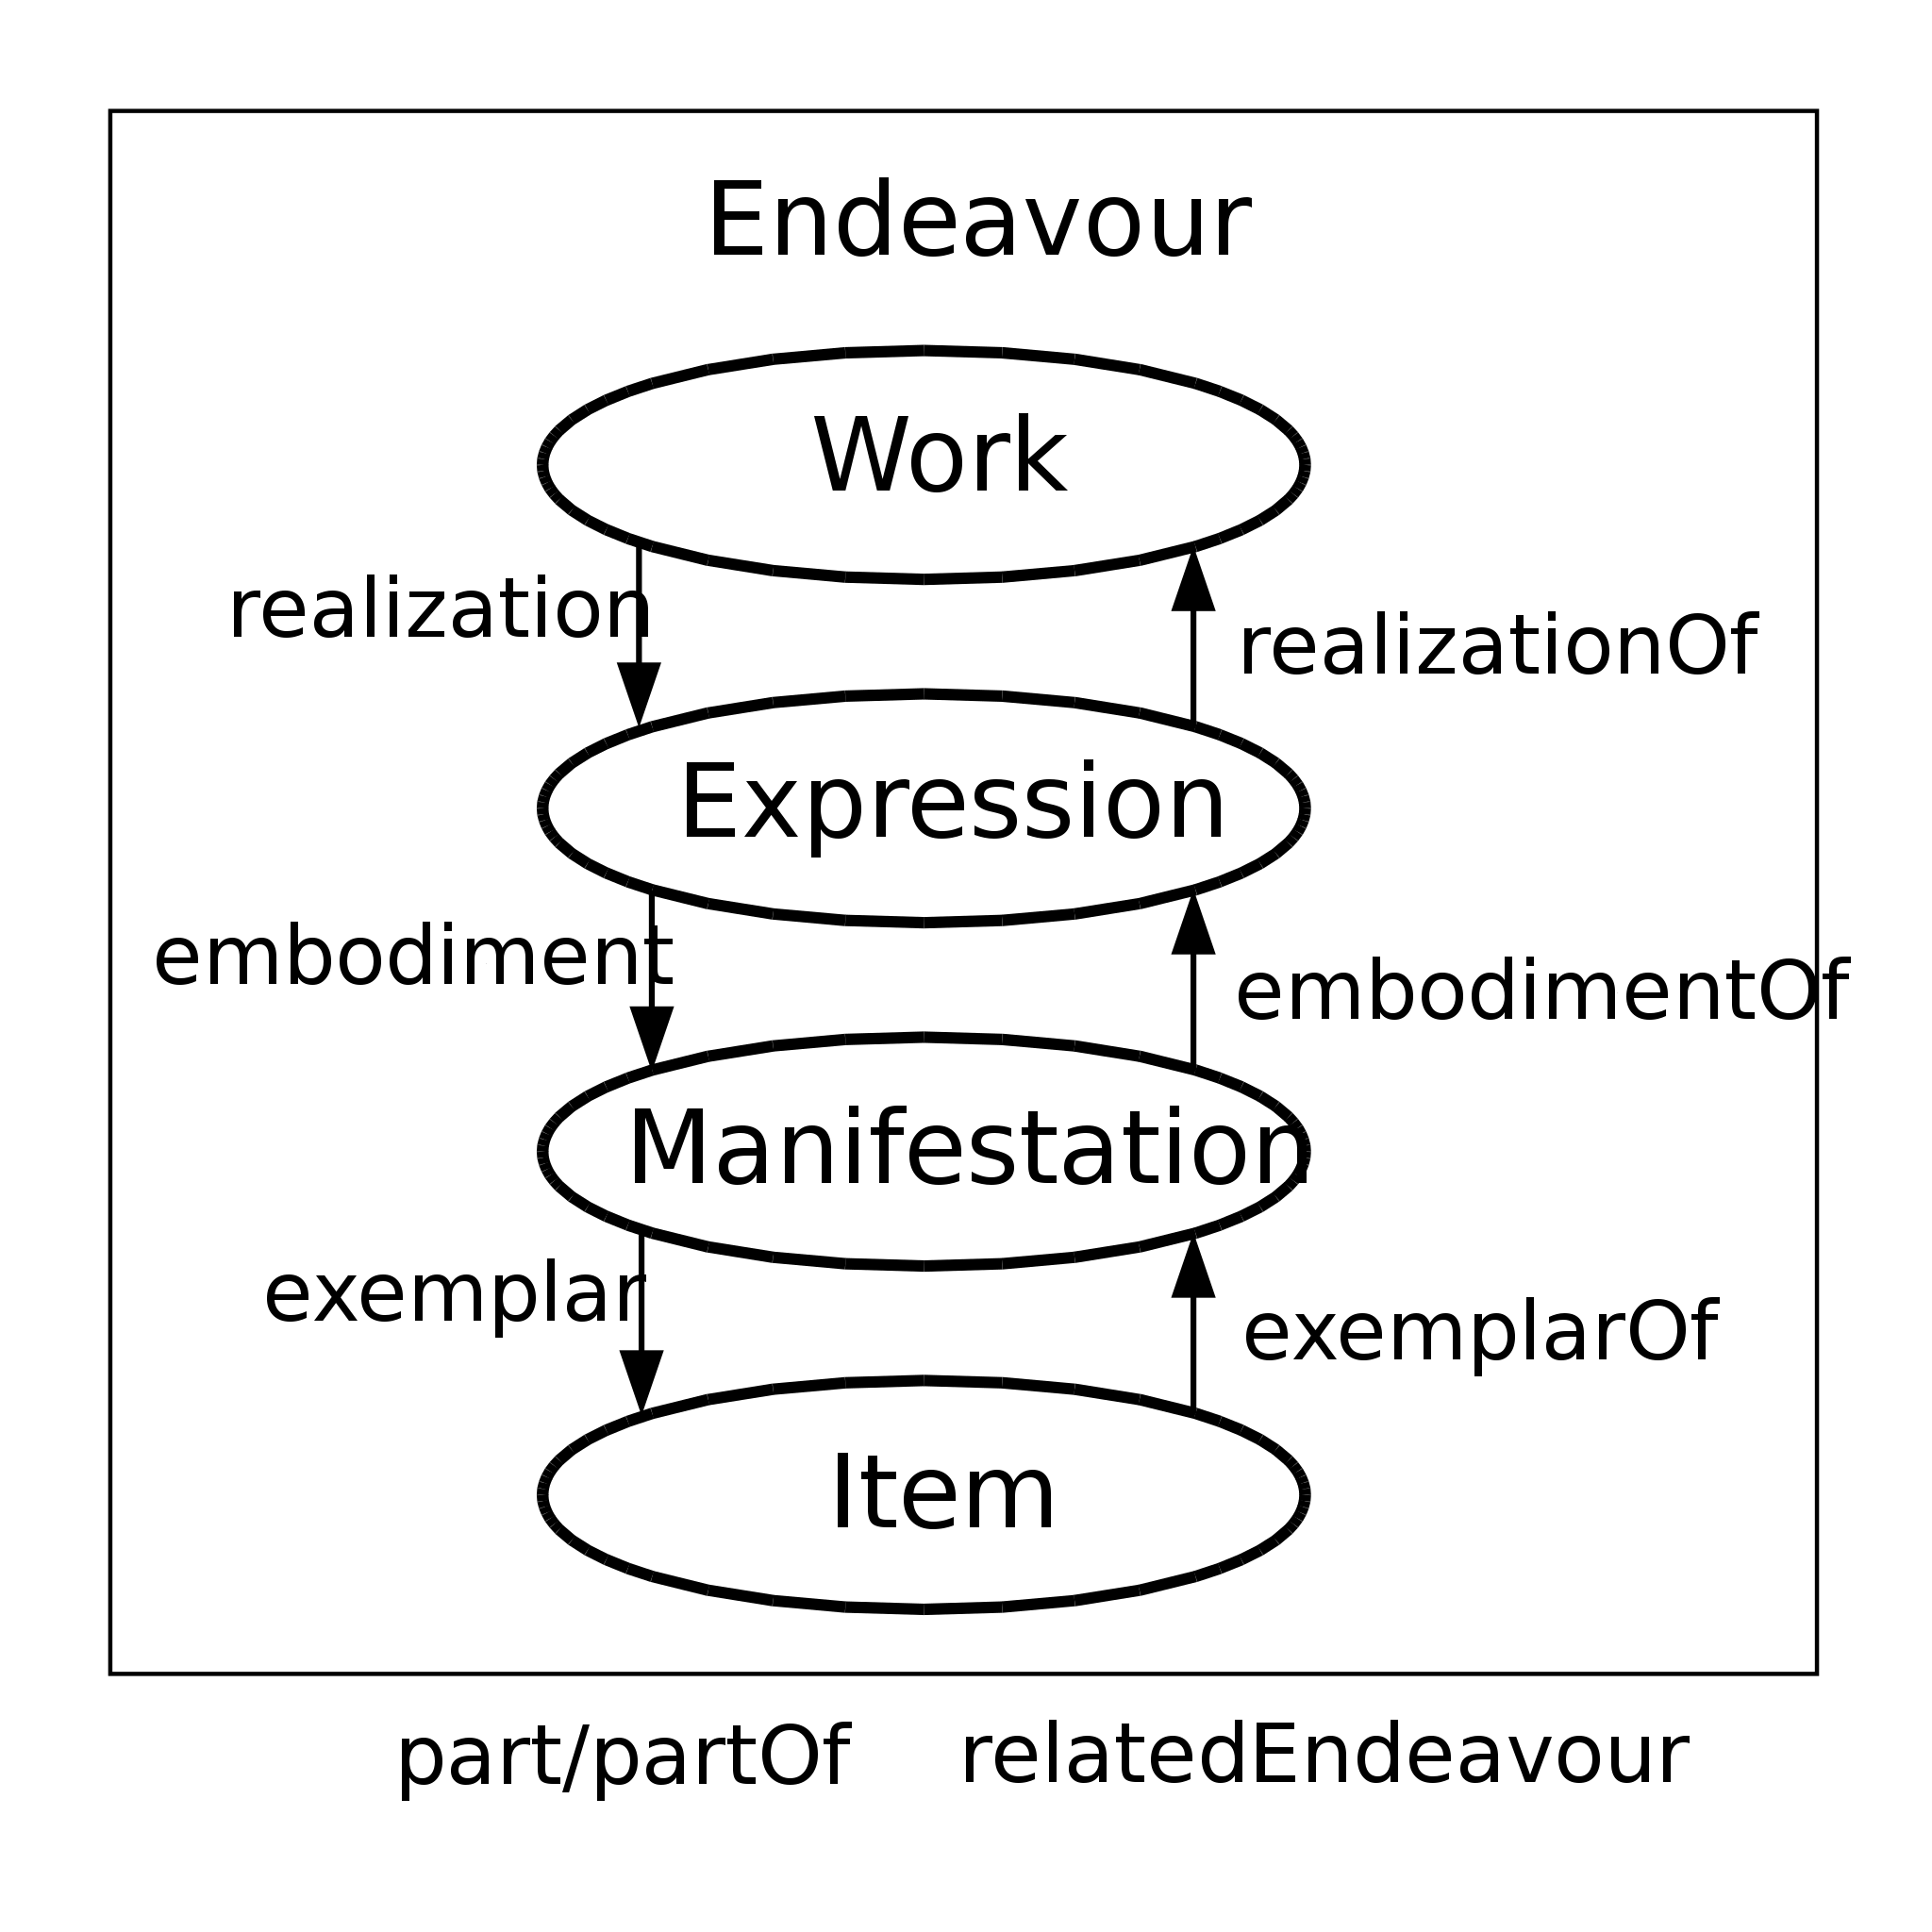
\includegraphics[height=60mm]{img/FRBR_Group1.png}
  \qquad
  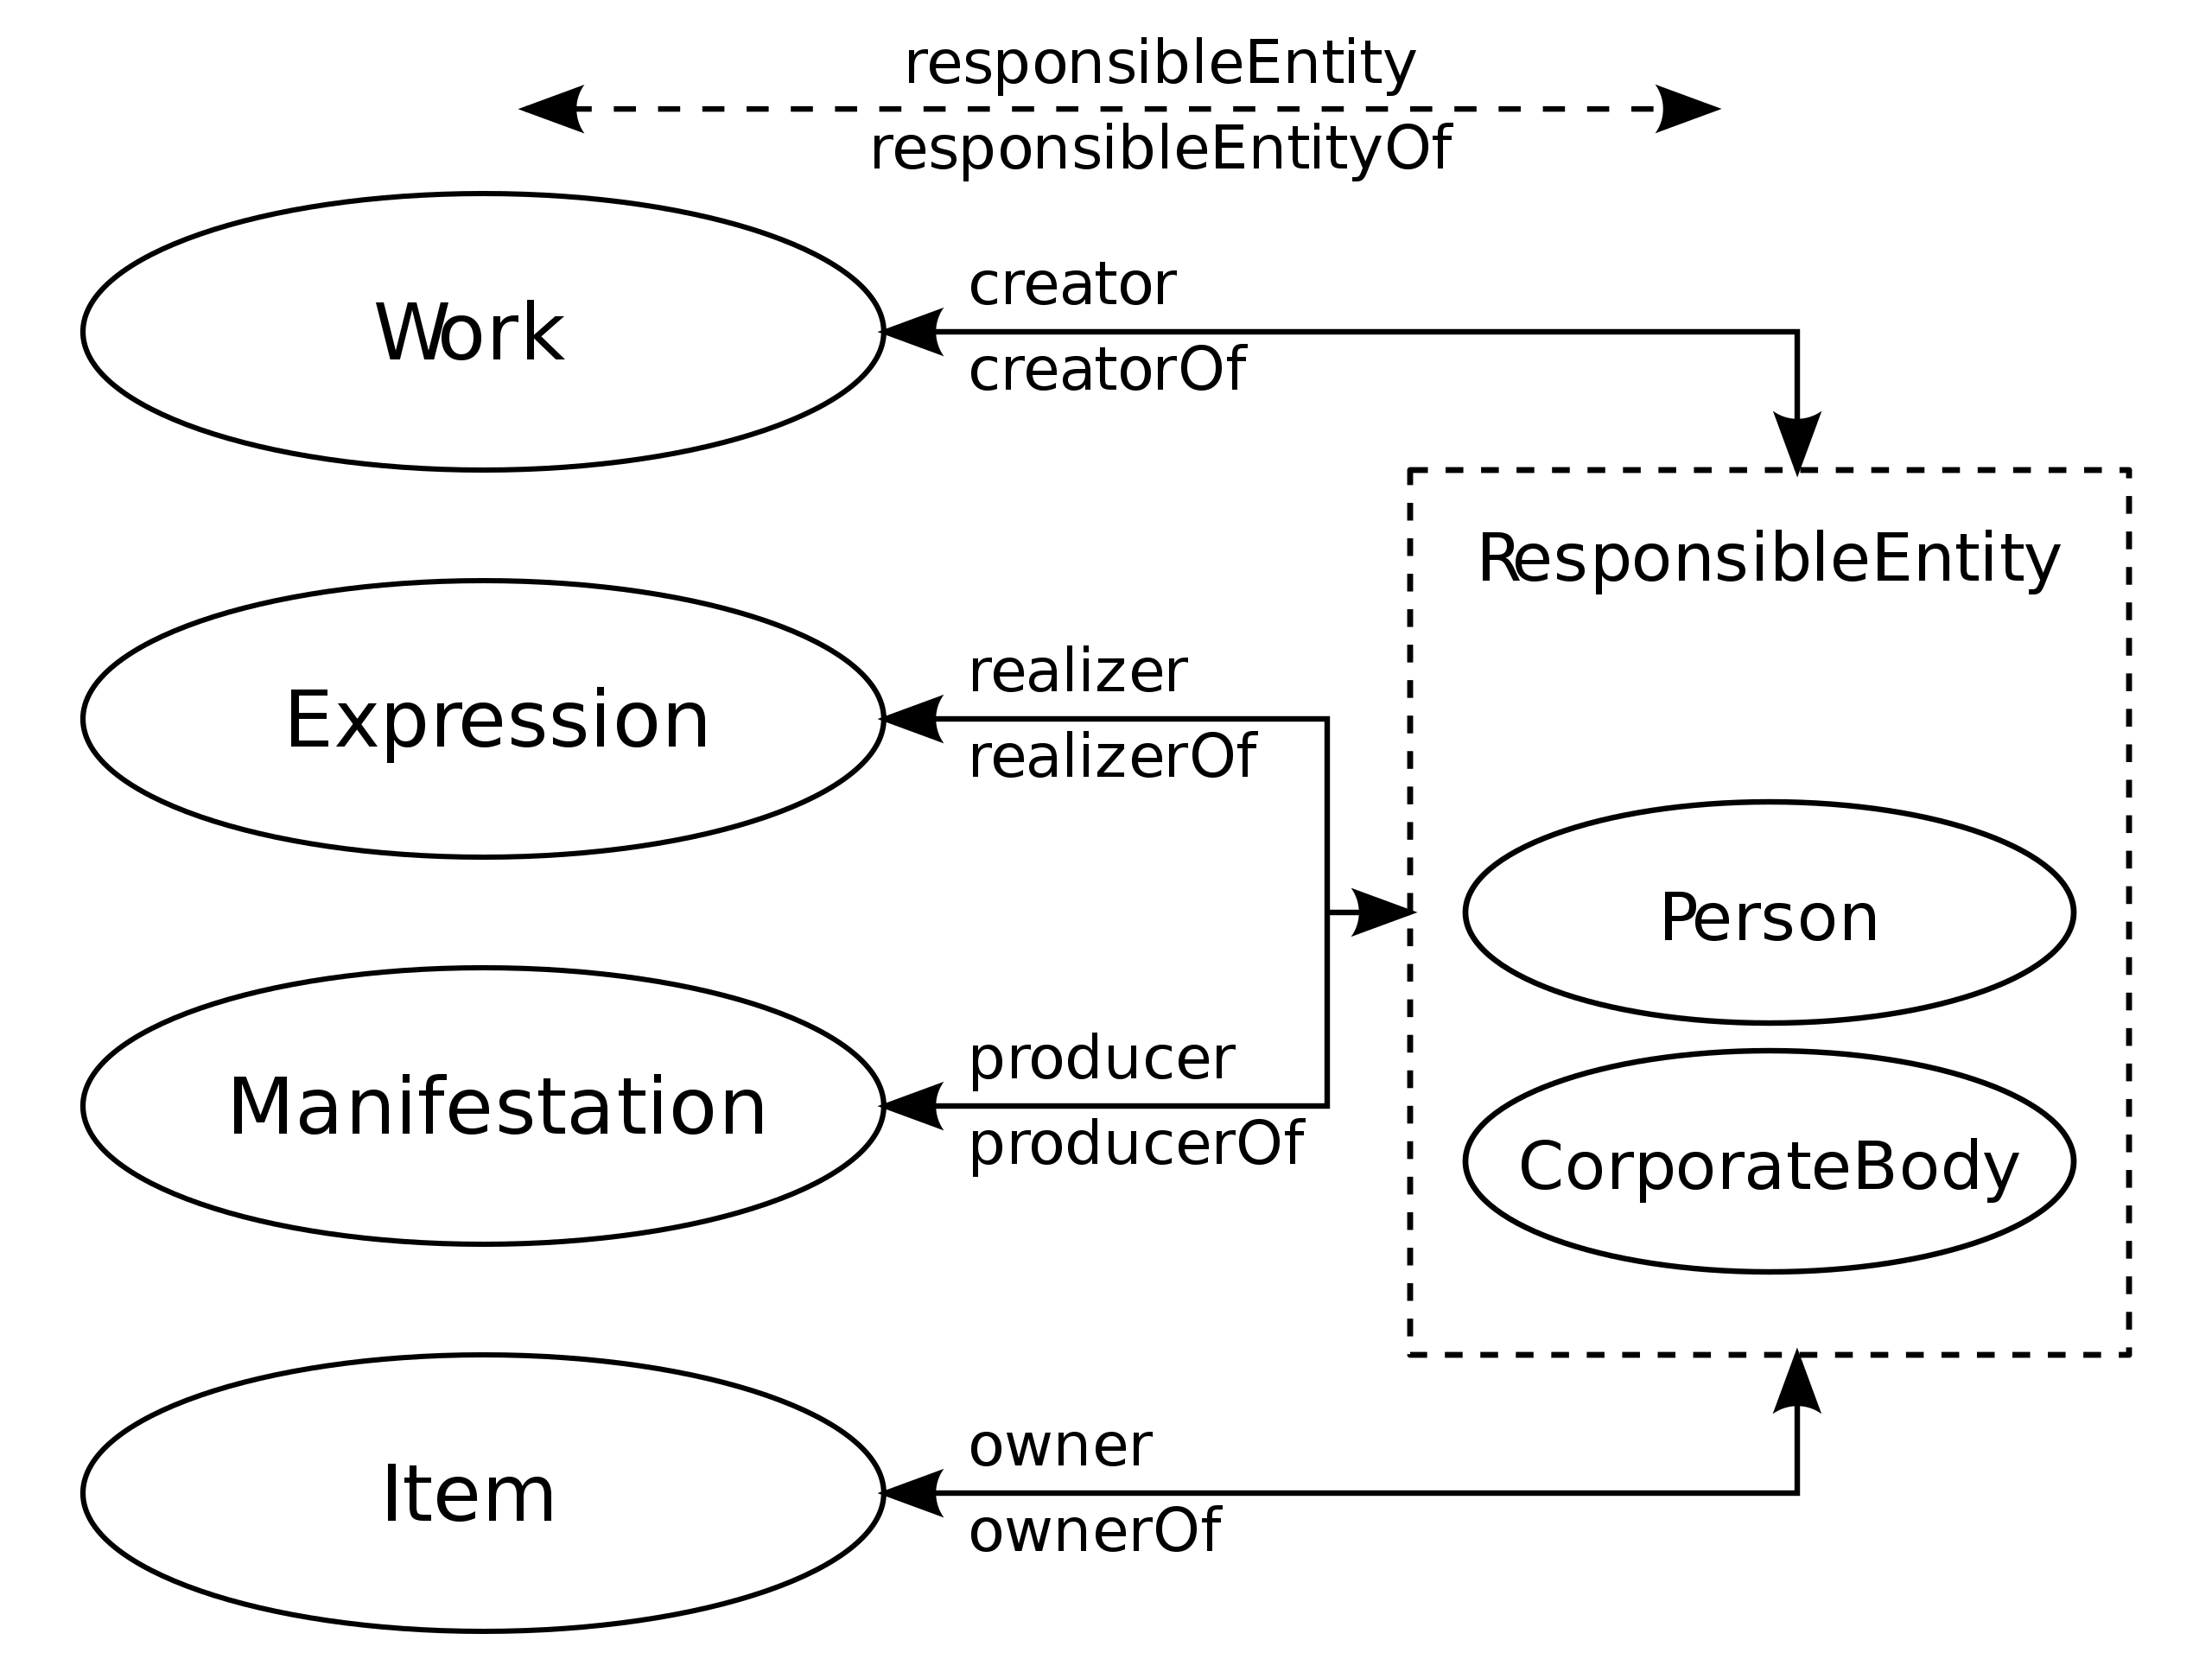
\includegraphics[height=60mm]{img/FRBR_Group2.png}
  
  \caption[Basic FRBR entities and relations of Group~1 and Group~2]{%
    \parbox[t]{.85\linewidth}{%
      Basic \gls{FRBR} entities and relations of Group~1 (left) and Group~2 (right)
      \par
      \begin{footnotesize}
        \href{https://commons.wikimedia.org/wiki/File:FRBR-Group-1-entities-and-basic-relations.svg}{\enquote{Basic Group 1 entities and relations of the FRBR model (RDF version)}} and
        \href{https://commons.wikimedia.org/wiki/File:FRBR-Group-2-entities-and-relations.svg}{\enquote{Basic Group 2 entities and relations of the FRBR model (RDF version)}}
        by \href{https://commons.wikimedia.org/wiki/User:JakobVoss}{Jakob Voss} are licenced under \href{https://creativecommons.org/licenses/by-sa/4.0/}{CC BY-SA 4.0}.
        \par
      \end{footnotesize}
    }%
  }
  \label{fig:FRBR}
\end{figure}

FRBR serves as a basic principle of RDA, which we discuss in the following.

% .............
\paragraph{RDA}

\dots


\begin{itemize}
  \item 
    \mybold{OPAC or K10plus data model as ER diagram? Binary vs. \boldmath$n$-ary relations?
    $\leadsto$ check literature (possibly also papers on the FRBR model)!}
  \item
    SRU: \url{https://en.wikipedia.org/wiki/Search/Retrieve_via_URL}, \url{https://www.loc.gov/standards/sru/}
\end{itemize}

\dots


% -----------------------------------------------------------------
\section{Data Sources}
\label{sec:data_sources}

We have searched the literature and the Web for data sources that contain information
relevant for provenance research, i.e., works, expressions, manifestations, exemplars,
persons, ownership, social relationships, and more. 
We decided to put a slight focus on data sources from the German-speaking area, 
aiming at a selection of data sources that is manageable in the context of a master's thesis,
and influenced by the selection in the \gls{SoNAR} project (see Section~\ref{sec:HNA+SoNAR}).
In the following, we will first give an overview of these data sources
and then provide more information about some of them,
including their scope and the technical infrastructure provided.
This list is not exhaustive and needs to be extended
as soon as our model is implemented in a concrete tool in future work.

% - - - - - - - - - - - - - - - - - - - - - - - -
\subsection{Collection of Data Sources}

We have identified four categories of relevant data sources:
library catalogues, special databases for provenance research, authority files, and knowledge bases.
We next describe, for each of these categories, the relevant information that is
contained in the respective data sources, and we list examples.

% .............
\paragraph{Library Catalogues}
%
%Library catalogues 
contain the following information relevant for provenance research.
%
\begin{itemize}
  \item
    bibliographic entities (works, manifestations, expressions, exemplars)
  \item
    relations between these entities (e.g., \term{isManifestationOf})
  \item
    attributes for these entities (e.g., year of publication)
  \item
    people and corporate bodies and relations such as authorship
  \item
    provenance entries (including, e.g., owners, the ownership relation, and further attributes such as the year of ownership)
  \item
    (implicitly) the current ownership
  \item
    (ideally) references to entries in authority files for all these types of entities
\end{itemize}
%
Examples of relevant library catalogues include:
%
\begin{itemize}
  \item
    catalogues of national libraries, which often aim at collecting literature exhaustively
    and which are most likely to make metadata available in interoperable formats;
    in particular: \gls{DNB}, \gls{LoC}, British Library
  \item
    meta-catalogues that enable a federated search in several catalogues;
    in particular: WorldCat and \gls{KVK}
  \item
    catalogues of (German) library networks;
    in particular: \gls{K10plus}, 
    \glsunset{B3KAT}\gls{B3KAT},
    \glsunset{hbz}%
    \glsunset{hebis}%
    and the union catalogues of \gls{hbz} and \gls{hebis}
  \item
    catalogues of single libraries, if not covered by any of the above
  \item
    special catalogues;
    in particular: \gls{ZDB}, \gls{KPE}, \gls{ZEFYS}, ExilePress (which have been used in the \gls{SoNAR} project) \todo{explain; relate to SoNAR or loot research}
\end{itemize}

% .............
\paragraph{Authority Files}
%
%Authority files
contain the following information relevant for provenance research.
%
\begin{itemize}
  \item
    entities such as persons, corporate bodies, places, works
  \item
    relations such as social relations, family relations, professional relations
  \item
    attributes for the entities such as their profession
\end{itemize}
%
They are usually subject to a strict quality control.
Examples include the \gls{GND} in the German-speaking area (which has been used extensively in \gls{SoNAR}),
the \gls{LCNAF} for North America,
and \gls{ISNI} and \gls{VIAF} worldwide.

% .............
\paragraph{Knowledge Bases.}

According to the insights from the \gls{SoNAR} project,
(open) \glspl{KB} can be useful when trying to overcome the problem with missing or unbalanced data
in authority files such as the \gls{GND} (see Section~\ref{sec:HNA+SoNAR}).
\Glspl{KB} are usually edited independently of the library domain by a wider community of contributors,
and their quality cannot be expected to meet the standards of catalogues or authority files edited by library personnel.
A prominent example of an open, cross-domain \gls{KB} is Wikidata,
which has tentatively been used in the context of the \gls{SoNAR} project.

% .............
\paragraph{Cultural Heritage Databases.}

This category contains generic federated portals of cultural heritage items
as well as special databases created especially for the support of provenance research.
Examples for these two kinds of databases are, respectively, Europeana (see Section~\ref{sec:linked_data+integration})
and Proveana---the research database of the German Lost Art Foundation \autocite{Proveana}.

% - - - - - - - - - - - - - - - - - - - - - - - -
\subsection{Analysis of Data Sources}

We now provide a review of the following data sources from the previous list:
\gls{DNB}, \gls{KVK}, \gls{K10plus}, \gls{ZDB}, \gls{KPE}, \gls{GND}, Wikidata, Proveana, and Europeana.
The main goal of this analysis is to provide an exemplary overview of the features and specifics
of these data sources, and to inform the model that we will develop in the subsequent chapter.
In order to fulfil this purpose, it is not necessary to review all data sources listed above
exhaustively.

We collect the following information for each data source.
%
\begin{itemize}
  \item
    \emph{Scope:}~
    thematic focus; coverage; number of records; standards for cataloguing
  \item
    \emph{Technical infrastructure:}~
    data format; data model; interfaces; support for linked data
  \item
    \emph{Data quality (from the \gls{SoNAR} grant proposal \autocite[p.\,19ff.]{SchneiderKempf2018}),
    if applicable:}~
    use of persistent identifiers and URIs; adherence to standards for, e.g., time and date specification
  \item
    \emph{features useful in the context of \gls{SoNAR} (see our discussion in Section~\ref{sec:insights_from_SoNAR}), if applicable:}~
    recording of temporal attributes or relations; recording of data provenance
  \item
    further features specific to the respective data source, if applicable
\end{itemize}

% .............
\paragraph{DNB.}

The following information is taken from the \gls{DNB}'s websites under the category \enquote{DNB Professional} \autocite{DNB_coll_mand,DNB_cataloguing,DNB_metadata}.

The DNB adheres to a legal collection mandate, according to which
the DNB collects \enquote{all texts, images and sound recordings published in Germany or in the German language, translated from German or relating to Germany that have been issued since 1913}  \autocite{DNB_coll_mand}. This includes all physical publications, and, since 2006, electronic publications made available via the internet. The mandate commits the DNB to a complete and unbiased collection that includes, among others, \enquote{printed works compiled or published between 1933 and 1945 by German-speaking emigrants} \autocite{DNB_coll_mand}.

The DNB catalogues its entire collection both descriptively and by subject, 
adhering to standards such as \gls{RDA}, using authority data, and including persistent identifiers such as ISBN, ISSN, URN, and DOI.
The cataloguing data feeds the German National Bibliography.

According to the 2021 annual report \autocite{DNB_Jahresbericht_2021},
the DNB's holdings comprise 43.7 million physical or digitally accessible units, 
which are represented by almost 26 million records in the German National Bibliography.

Metadata can be obtained from the DNB freely (under the CC0 1.0 licence) via the interfaces
\gls{SRU} and \gls{OAI}, which support XML serialisations of the data formats
MARC~21, \gls{RDF}, DNB Casual (an XML-based Dublin Core format), and MODS.\todo{introduce all these abbreviations}
Further data formats are available via an individual access
to the \enquote{Data Shop}.
The DNB's Linked Data Service provides open access to its bibliographic and authority data
in RDF under the Creative Commons Zero (CC0 1.0) license. Instructions on how to use these interfaces
are given on the DNB's webpage on metadata services \autocite{DNB_metadata}.

According to the detailed specifications on the MARC format by the DNB
\autocite{DNB_MARC21,DNB_MARCXML}, the recording of dates and times, languages,
geographic area codes, and countries conforms to ISO standards (8601, 639-1, 3166).
Since 2015, the DNB has been using MARC field 883
for recording the metadata provenance for a selection of data fields
\autocite{DNBwiki_MARC_883}.

RDA and the application guidelines for the German-speaking area
stipulate the following practice for cataloguing works, expressions, manifestations, and exemplars
in relation with each other: Bibliographic records (\enquote{Titeldatensätze})
have a bibliographic level for describing a manifestation
and an exemplar level for describing the related exemplars. The description of works and expressions
is considered part of the description of a manifestation and thus recorded on the bibliographic level.
However, it is possible to create and link an authority record for a work or expression
containing the relevant description. In that case, the source of the information can be recorded as well
\autocite[cf.][Chapter~5.1]{Wiesenmueller2015}.

\todo[inline]{temporal data restricted to year of publication?}

% .............
\paragraph{WorldCat}

\dots

% .............
\paragraph{KVK}

\dots

% .............
\paragraph{K10plus}

is the joint catalogue of the German library networks GBV and SWB.
Together, these two networks comprise more than 1400 national, regional,
academic, and public libraries \autocite{BSZGBV,GBV_VZG},
of which 838 participate in K10plus, according to the list of participating institutions
in the K10plus Wiki \autocite{K10plusWiki}. Thus, \gls{K10plus} comprises the data from
the majority of German academic institutions \autocite[cf.][]{BSZ_K10plus}.

Cataloguing in K10plus adheres to the same standards as in the DNB.
As of 31 December 2022, K10plus contains 80.8 million bibliographic records (\enquote{Titeldatensätze})
with 235.4 million ownership records \autocite{GBV_K10plus_Statistik}.

K10plus provides metadata freely (under the CC0 1.0 licence),
mainly via the interfaces Z39.50 and SRU.
Those support the data formats MARC~21, MARC-XML (and its variant Turbomarc),
PICA+, PICA-XML, DC, and MODS (and the legacy format MAB2).
Detailed instructions on how to use these interfaces
are given in the K10plus Wiki \autocite{K10plusWiki}.
In addition, snapshots of K10plus data are provided regularly
in MARC-XML and as LOD (RDF-XML), but the information
on these in the K10plus Wiki is incomplete \autocite{K10plusWikiOD}.



\dots

\todo[inline]{discuss provenance indexing}

\todo[inline]{GND data accessible via the same interface? Prepare for GND section below}


% .............
\paragraph{ZDB}

\dots

% .............
\paragraph{KPE}

\dots

% .............
\paragraph{GND.}

The \gls{GND} is operated by the \gls{DNB}
\enquote{in cooperation with many other libraries, libra[r]y networks and other cultural and academic institutions.
At present, the GND contains around 9 million authority records for persons, corporate bodies, congresses, geographic entities, specialised terms and works; these are supplemented, updated and used frequently} \autocite{DNB_cataloguing}. More detailed statistics can be found in the DNB's
2021 annual report \autocite[p.49]{DNB_Jahresbericht_2021}.
GND adheres to the same cataloguing standards and offers the same technical infrastructure
as the DNB catalogue; in particular, GND data is accessible alongside DNB data
via the same interfaces and data formats, including RDF.

\todo[inline]{temporal data restricted to year of publication or years of birth and death, if available? No temporal attributes on relations (e.g., student, coauthor) $\Longrightarrow$ first review K10plus guidelines for cataloguing authority data!}


\todo[inline]{add insights from SoNAR (§~\ref{sec:HNA+SoNAR}) and DHa (see below)}

DHa's remarks on GND vocabulary and richness of GND data:
%
\begin{itemize}
  \item
    \emph{Individualisierungsregeln}: relationships to other people are given in order to uniquely
    identify the current person; there is no obligation to record relationships
    (and GND does not claim to be an encyclopedia)
  \item
    relations are not normed:
    e.g., field \enquote{Funktionsbezeichnung}: \$4 code \enquote{Eigenschaft der Beziehung},
    specified by \$v \enquote{Freitext}
  \item
    professions are recorded in 678 \$b \enquote{biographische Anmerkung(en)} --
    historically in free text,
    more recently via link to the GND authority data for the respective profession (i.e., more standardised)
  \item
    Tp1 datasets: field 65 (6J?) \enquote{GND Systematik: eingeschr. Tätigkeit} (?),
    query level 1 datasets?
  \item
    $\leadsto$ \mybold{look/read all this up!}
\end{itemize}


\dots


% .............
\paragraph{Wikidata}

\dots

% .............
\paragraph{Proveana}

\dots

% .............
\paragraph{Europeana}

\dots

\par\bigskip
\todo[inline]{Take the following points into account ::}

\begin{itemize}
  \item
    \mybold{KVK} (\enquote{federated search}: shallower than in single catalogues,
    but (sufficient) information on all copies!);
    further catalogues?
  \item
    more from \gls{SoNAR} , see report on WP 2 (in particular details on p.23f.).
    Get back to the discussion on \gls{GND} and further data sources in Section~\ref{sec:HNA+SoNAR}.
  \item
    see also the list by \autocite{Menzel2020}:

    \blockquote{%
      \begin{itemize}
        \item
          The Integrated Authority File (GND) represents and describes 8,295,047 entities (people, corporations, conferences, geographical areas, technical terms, and works);
        \item
          The German National Library (DNB) provides descriptions of bibliographic resources. The dataset has 19,926,573 records of books, magazines, newspapers, sheet music, music recordings, audio books etc.;
        \item
          The German Union Catalogue of Serials (ZDB) describes newspapers, magazines, serial titles, yearbooks, etc. and contains 1,908,334 records;
        \item
          The Kalliope Union Catalog (KPE) is a collection of personal papers, manuscripts, and publishers’ archives, which consists of 26,752 records;
        \item
          The Newspaper Information System (ZeFYS) represents 2,596,641 digitized pages of historical newspapers and full texts;
        \item
          The Exile Press represents German-language exile journals between 1933 and 1945 and consists of 5,336 digitized pages.
      \end{itemize}
    }
  \item
    further criteria: arity of relationships, data formats, temporal data?
  \item
    also clarify: does the structure of these data sources support the model to be developed?
  \item
    focus the following considerations on a narrow choice of these data sources;
    the general approach to be developed should be largely independent on that concrete choice
  \item 
    in-depth analysis of data sources (e.g., overlap and differences) is worthwhile
    but must be deferred to future work
\end{itemize}

% -----------------------------------------------------------------
\section{Data Integration and Further Techniques}
\label{sec:data_integration}

\begin{itemize}
  \item 
    ETL (from grant proposal \gls{SoNAR}, p.~8, AP1-1)
  \item
    upper-level ontologies?
  \item 
    ontologies on research
  \item
    FRBRoo?
  \item
    \gls{RDF}, SPARQL, N-Quads?
\end{itemize}


\dots

% -----------------------------------------------------------------
\section{Implications on Modelling}
\label{sec:implications_on_modelling}

\dots

\begin{itemize}
  \item
    \mybold{constants plus unary and binary relationships suffice (?) -- evidence: FRBR, works on graph techniques in HNA, data sources}
  \item 
    online vs.\ offline phase?
    %
    \begin{itemize}
      \item
        online: data source graph is implicit; data sources are queried \enquote{on the fly}
      \item
        offline: data source graph is generated explicitly (using data integration techniques)
        and updated in fixed intervals
    \end{itemize}
    %
\end{itemize}



  % !TeX spellcheck = en_GB
% =================================================================
\chapter{Modelling Provenance Relationships}
\label{chap:modelling}

\todo[inline,color=red!30]{Give more explanation for people not familiar with graph theory; make steps that seem logical more explicit; name advantages of using graph theory as an instrument (modelling power, abstraction, available methods, well-behaved algorithms, ready-to-use implementations); span bridge from concrete example queries to GT; possibly give links to basic (video) tutorials in GT (ask Leif?)}
  
In this chapter, we develop a generic approach to modelling provenance relationships.
More precisely, we need to model three central notions: queries that a user may want to ask,
data sources that are to be consulted in order to answer a query,
and answers given to a query.
In order to obtain a generic approach, we aim at providing rigorous definitions
for these central concepts, and we seek intensional rather than extensional definitions.
In particular, those definitions should not depend on concrete example queries or data sources
such as the ones discussed in Chapters~\ref{chap:prototype_queries} and~\ref{chap:analysis};
neither should they depend on concrete objects, concepts, or relationships
(such as \enquote{Copernicus}, \enquote{exemplar}, or \enquote{student}).
Instead, we will develop an abstract model with precise but general definitions
of the notions of a query, data source, and answer.
This model can then be used with a multitude of concrete queries and data sources,
and its potential implementation will provide answers as specified by our definitions.

\todo[inline]{Discuss the choice of this graph-based framework; delineate from classical database theory (text snippets commented out). This argument should be a logical consequence of the requirement analysis in the previous chapter(s)!}
%An obvious choice would be to base our abstract model on database theory,
%where the notions of a database, a query, and a query answer are well-defined based on rigorous mathematical concepts;
%see, e.g., the standard introduction ... \todo{citation}.
%This framework is very general, well-established, and implemented in database management systems
%that scale well to large databases \todo{citation}.
%However, .....
%...
%We want to model individuals and concepts (e.g., ...) as well as relationships
%between individuals (e.g., ...).  $\leadsto$ constants, unary and binary relations
%...
%With the choice of graphs, we commit ourselves to a restricted view of a data source:
%graphs can only represent unary and binary relations via nodes and edges
%while, in general, a database may have relations of arbitrary arity.
%However, we do not consider this a significant restriction in the context of our purpose
%because we only want to represent relations that are relevant for provenance research,
%and those are predominantly unary or binary. \todo{strengthen argument, give examples, consult literature}
%
%%
%\begin{itemize}
%  \item
%    mathematically complex
%  \item
%    hard to visualise
%  \item
%    relations of arity $\geqslant 2$ seem overkill, given the relations used in OPACs, GND, Wikidata
%\end{itemize}
%%
%\todo[inline]{We first need an analysis of available data sources and of requirements; only then can we justify the choice of framework.}

As 
\todo{this par is tentative}
a central notion for representing data sources
and queries, we use directed graphs with labels.
The concept of a graph is widely used in computer science and discrete mathematics;
see standard textbooks \autocite[e.g.,][]{Diestel2012}.
Graphs and graph techniques are used to represent large knowledge bases \autocite[e.g.,][]{Ehrlinger2016}.
They provide an easy means for visualising objects and their relationships,
and they lend themselves to computationally well-behaved algorithms for query answering. \todo{explain; citation}

\todo[inline,caption={}]{
  \parbox{.99\linewidth}{%
    Comment on restrictions made:
    %
    \begin{itemize}
      \item
        no temporal distinctions (\enquote{is/was student}) or \enquote{was owner in year $n$}. 
      \item[$(\leadsto)$]
        no attributes for relationships (citation)
      \item[$\leadsto$]
        keep the presentation digestible for readers with little or no background in maths and CS
        (i.e., a large proportion of librarians and historians).
      \item
        possible extensions in Section~\ref{sec:possible_extensions}
    \end{itemize}
  }%
}

% -------------------------------------------------------------------
\section{Labelled Directed Graphs}
\label{sec:labelled_digraphs}

In a nutshell, a labelled directed graph consists of a set of nodes, a set of directed edges between
the nodes, a function that names nodes with individuals,
and a function that labels the nodes (edges) with concepts (relations)
of which the nodes (edges) are instances.
In our setting, these four abstract components have the following meaning:
%
\begin{itemize}
  \item 
    Nodes represent entities such as works, expressions, manifestations, items,
    persons, or corporations.
  \item 
    Edges represent relationships between nodes, which are typically directed:
    e.g., \term{has\_owner} points \emph{from} an item
    \emph{to} a person or corporation,
    whereas \term{is\_owner\_of} points into the opposite direction.
    Symmetric relationships, such as \term{collaborates\_with},
    can be represented via two edges, one for each direction.
  \item 
    The unique node name specifies the individual that is represented by the node.
  \item 
    Node labels allow the specification of one or several concepts
    of which the respective node is an instance.
    For example, a node representing the physicist Albert Einstein
    may be labelled, among others, with the concepts \term{Person}, \term{Scientist},
    and \term{Physicist}.
%  \item 

    Edge labels allow the specification of one or several relation names for each edge.
    For example, if a person $p_1$ has a student $p_2$ and, in later life, 
    collaborates with $p_2$, then this can be represented via an edge from $p_1$ to $p_2$
    with the label $\{\term{has\_student},\term{collaborates\_with}\}$
    (and/or an edge from $b$ to $p$ with the label $\{\term{is\_student\_of},\term{collaborates\_with}\}$).
\end{itemize}
%
A labelled directed graph can be visualised in the obvious way:
each node is represented using a circle or rectangle
enclosing the node's name,
and each edge is denoted by an arrow.
Node and edge labels are written next to the respective node or edge;
multiple labels of the same node or edge are delimited with commas.
An example is given in Figure~\ref{fig:example_graph},
which represents a part of the data described in Chapter~\ref{chap:prototype_queries}
concerning an exemplar of Copernicus' \emph{De revolutionibus} at the
Gotha Research Library \emph{(FB Gotha)}.
For the sake of simplicity, the example graph deviates from the FRBR model
by omitting the FRBR entities \enquote{Expression} and \enquote{Manifestation}
between the nodes labelled \enquote{Work} and \enquote{Item}.

\newcommand{\tikzexagraph}[1][]{%
  \node [#1]                                (work1)   {\fns\tikztab{\term{De revolutionibus}}};
  \node [below=21mm of work1]               (item1)   {\fns\tikztab{\term{FB Gotha}\\[-1pt]\term{Druck~4°~00466}}};
  \node [above right=4mm and 50mm of work1] (person1) {\fns\tikztab{\term{Nicolaus}\\[-1pt]\term{Copernicus}}};
  \node [above right=9.5mm and 50mm of item1] (person2) {\fns\tikztab{\term{Johann}\\[-1pt]\term{Hommel}}};
  \node [below right=9.5mm and 50mm of item1] (person3) {\fns\tikztab{\term{Valentin}\\[-1pt]\term{Thau}}};
  
  \begin{scope}[%
    every node/.style={draw=none,fill=none,inner sep=.2mm}
  ]
    \path[->]
      (work1)   edge[bend right=10] node[pos=.4,left=1mm]      {\fns\tikztab[r]{\term{has\_}\\[-1pt]\term{exemplar}}} (item1)
      (item1)   edge[bend right=10] node[pos=.8,right=1mm]     {\fns\term{is\_exemplar\_of}}      (work1)
      (work1)   edge[bend left=4]   node[pos=.5,sloped, above] {\fns\strut\term{has\_creator}}    (person1)
      (person1) edge[bend left=4]   node[pos=.5,sloped, below] {\fns\strut\term{is\_creator\_of}} (work1)
      (item1)   edge[bend left=14]  node[pos=.5,sloped, above] {\fns\strut\term{has\_owner}}      (person2)
      (person2) edge[bend right=6]  node[pos=.5,sloped, below] {\fns\strut\term{is\_owner\_of}}   (item1)
      (item1)   edge[bend right=6]  node[pos=.5,sloped, above] {\fns\strut\term{has\_owner}}      (person3)
      (person3) edge[bend left=14]  node[pos=.5,sloped, below] {\fns\strut\term{is\_owner\_of}}   (item1)
      (person2) edge[bend right=10] node[pos=.46,left=1mm]     {\fns\tikztab[r]{\term{has\_student,}\\[-1pt]\term{collaborates\_with}}} (person3)
      (person3) edge[bend right=10] node[pos=.54,right=1mm]    {\fns\tikztab{\term{is\_student\_of,}\\[-1pt]\term{collaborates\_with}}} (person2)
    ;
      
    \node[above=.5mm of work1]   () {\fns\term{Work}};
    \node[below=.5mm of item1]   () {\fns\term{Item}};
    \node[right=.5mm of person1] () {\fns\tikztab{\term{Person,}\\[-1pt]\term{Scientist}}};
    \node[right=.5mm of person2] () {\fns\tikztab{\term{Person,}\\[-1pt]\term{Mathematician}}};
    \node[right=.5mm of person3] () {\fns\tikztab{\term{Person,}\\[-1pt]\term{Astronomer}}};
    
  \end{scope}      
}
%
\begin{figure}[ht]
  \centering
  \begin{tikzpicture}[
    >=Latex,
    every node/.style={on grid,rectangle,rounded corners=1mm,draw=black,fill=lightblue,thick,inner sep=1.5mm},
    every edge/.style={draw=black,thick}
  ]
    \tikzexagraph
  \end{tikzpicture}
  
  \caption{An example graph}
  \label{fig:example_graph}
\end{figure}

As we will see in the following, labelled directed graphs can be used in our setting
to represent (combinations of) data sources as well as queries.
They allow us to draw on standard notions from graph theory and query answering
in order to define admissible query answers and to devise methods for obtaining those.

These considerations lead to the following definition of a labelled directed graph.

%\begin{definition}
%  Let $R$ be a set of \emph{relation names}.
%  A \emph{directed edge-labelled graph over $R$} is a triple $G = (V,E,\Lmc)$,
%  where
%  %
%  \begin{itemize}
%    \item
%    $V$ is a set, whose members are called or \emph{nodes};\footnote{%
%      In classical graph theory, nodes are called \emph{vertices}; thus the set of
%      nodes of a graph is denoted by $V$. We adopt the denotation $V$ for conformity
%      and the more modern term \enquote{node} for brevity.%
%    }      
%    \item 
%    $E \subseteq V \times V$ is a set of pairs of nodes, whose members are called \emph{edges};
%    \item
%    $\Lmc : E \to 2^R$ is a function that assigns to each edge a non-empty set of relation names,
%    called the \emph{labels} of that edge; we call \Lmc a \emph{labelling function}.
%  \end{itemize}
%\end{definition}
%
\begin{definition}
  \label{def:ld_graph}
  Let $\namespace=(\NI,\NC,\NR)$ be a \emph{namespace} consisting of a set \NI of \emph{individual names}, a set \NC of \emph{concept names}, and a set \NR of \emph{relation names}.
  A \emph{labelled directed graph over $\namespace$} is a triple $G = (V,E,\Nmc,\Lmc)$
  where
  %
  \begin{itemize}
    \item
      $V$ is a set, whose members are called \emph{nodes};\footnote{%
        In classical graph theory, nodes are called \emph{vertices}; thus the set of
        nodes of a graph is denoted by $V$. We adopt the denotation $V$ for conformity
        and the more modern term \enquote{node} for brevity.%
      }      
    \item 
      $E \subseteq V \times V$ is a set of pairs of nodes, whose members are called \emph{edges};
    \item
      $\Nmc : V \to \NI$ is an injective function that assigns
      to each node a unique individual (called the node's \emph{name});
    \item
      $\Lmc : V \cup E \to \NV \cup 2^{\NR}$ is a function that assigns 
      to each node a set of concept names (called the node's \emph{labels}) and
      to each edge a non-empty set of relation names (called the edge's \emph{labels});
      we call \Lmc a \emph{labelling function}.
  \end{itemize}
\end{definition}
%
Definition~1 stipulates the following conditions.
%%
%\begin{itemize}
%  \item
%    every node has a unique name and no two nodes have the same name (the latter being ensured by injectivity);
%  \item
%    a node can have an arbitrary number of labels, including no label (in case the node belongs to no concept);
%  \item
%    an edge can have an arbitrary number of labels, but that number must not be zero --
%    the effect of an edge having no labels can be achieved by simply omitting the edge.
%\end{itemize}
%
(1) Every node has a unique name, and no two nodes have the same name (the latter being ensured by injectivity).
(2) A node can have an arbitrary number of labels, including no label (in case the node belongs to no concept).
(3) An edge can have an arbitrary number of labels, but that number must not be zero --
the effect of an edge having no labels can be achieved by simply omitting that edge.

In the example in Figure~\ref{fig:example_graph},
$V$ consists of five nodes, which we call $v_1,\dots,v_5$,
and $E$ consists of ten edges. Let $v_1,v_2$ denote the nodes on the left and $v_3,v_4,v_5$
denote the nodes on the right (both from top to bottom).
Then we have, among others, the following node names and labels:
%
\begin{equation*}
  \Nmc(v_1) = \term{work}_1
  \qquad
  \Lmc(v_1) = \{\term{Work}\}
  \qquad
  \Lmc(v_5) = \{\term{Person},\term{Astronomer}\}
\end{equation*}
%
Additionally, two of the ten edges have the following labels:
%
\begin{alignat*}{2}
  e_1 & = (v_4,v_5) & \qquad \Lmc(e_1) & = \{\term{has\_student},\term{collaborates\_with}\} \\
  e_2 & = (v_5,v_4) &        \Lmc(e_2) & = \{\term{is\_student\_of},\term{collaborates\_with}\} \\
\end{alignat*}

% ------------------------------------------------------------------
\section{Modelling Data Sources, Queries, and Answers}
\label{sec:modelling}

We now model a data source (e.g., library catalogue, authority file, or other database)
using the exact notion of a graph that we have introduced above.
%
\begin{definition}
  \scalebox{0.973}[1]{A \emph{data source over the namespace $\namespace=(\NI,\NC,\NR)$} is a labelled directed graph
  over \namespace.}
\end{definition}
%
%With this definition, we obviously commit ourselves to a restricted view of a data source:
%graphs can only represent unary and binary relations via nodes and edges
%while, in general, a database may have relations of arbitrary arity.
%However, we do not consider this a significant restriction in the context of our purpose
%because we only want to represent relations that are relevant for provenance research,
%and those are predominantly unary or binary. \todo{strengthen argument, give examples, consult literature}
%
In order to model queries with the same notion of graphs, we need to introduce
two sets of variables that serve as distinct node names:
For example, consider the following variant of the example query \exaquery{2} from Chapter~\ref{chap:prototype_queries}:
%
\begin{enumerate}
  \item[\exaquery{2$'$}]
%    Which exemplars of work $W$ were passed from one of its owners to a collaborator of theirs?
    Which exemplars of \emph{De revolutionibus} were owned by some scientist who passed them on to a student?
\end{enumerate}
%
Query~\exaquery{2$'$}
should be modelled by the graph shown in Figure~\ref{fig:graph_for_exa_query2'}.

\newcommand{\tikzexaquery}{%
  \node                                        (derev) {\fns\strut$\term{De revolutionibus}$};
  \node [ansvar,below=14mm of work1]           (x)     {\fns\strut$x$};
  \node [anovar,above right=6.4mm and 24mm of x] (y)     {\fns\strut$y$};
  \node [anovar,below right=6.4mm and 24mm of x] (z)     {\fns\strut$z$};
  
  \begin{scope}[%
    every node/.style={draw=none,fill=none,inner sep=.2mm}
  ]
    \path[->]
      (derev) edge node[left=1mm]           {\fns\tikztab[r]{\term{has\_}\\[-2pt]\term{exemplar}}} (x)
      (x)     edge node[sloped, above=.6mm] {\fns\term{has\_owner}}         (y)
      (x)     edge node[sloped, below]      {\fns\strut\term{has\_owner}}   (z)
      (y)     edge node[right=1mm]          {\fns\tikztab[r]{\term{has\_}\\[-2pt]\term{student}}} (z)      
    ;
      
    \node[above=.5mm of derev] () {\fns\term{Work}};
    \node[left=.5mm of x]      () {\fns\term{Item}};
    \node[above=.5mm of y]     () {\fns\term{Scientist}};
    
  \end{scope}
}
%
\begin{figure}[ht]
  \centering
  \begin{tikzpicture}[
    >=Latex,
    every node/.style={on grid,rectangle,rounded corners=1mm,draw=black,fill=lightblue,thick,inner sep=1.5mm},
    every edge/.style={draw=black,thick}
  ]
    \tikzexaquery
  \end{tikzpicture}
  
  \caption{A graph representing example query \exaquery{2$'$}}
  \label{fig:graph_for_exa_query2'}
\end{figure}

The nodes of this graph fall into three groups:
%
\begin{enumerate}[(1)]
  \item
    the node named \tikzinlinenode{\term{De revolutionibus}} represents that work;
  \item
    node \tikzinlinenode[ansvar]{$x$} represents an exemplar of this work that satisfies the conditions stated in~\exaquery{2$'$}
    and whose name is to be found;
  \item
    nodes \tikzinlinenode[anovar]{$y$} and \tikzinlinenode[anovar]{$z$}
    represent the two owners (scientist and their student) whose names are not known.
\end{enumerate}
%
Consequently, node name $x$ serves as a placeholder for the answer to the query,
and names $y,z$ are placeholders for further individuals that \enquote{witness} the answer.
We call $x$ the \emph{answer variable} and $y,z$ the \emph{anonymous variables}
of the query.

From now on, we fix two sets \VARANS and \VARANON
of \emph{answer variables} and \emph{anonymous variables}, respectively,
and we require that these two sets are disjoint with each other
and with any set \NI of individual names.
In particular, the namespace of data sources must not contain any variables,
in contrast to the namespace of queries.
These considerations lead to the following definition of a query.

\begin{definition}
  A \emph{query over the namespace $(\NI,\NC,\NR)$} is a labelled directed graph
  over $(\NI \uplus \VARANS \uplus \VARANON, \NC, \NR)$.
\end{definition}
%
\todo[inline,caption={}]{%
  Possibly comment on:
  %
  \begin{itemize}
    \item
      the special case of Boolean queries?
    \item
      specific requirements for modelling \exaquery{1} and \exaquery{3}: 
      \begin{itemize}
        \item 
          \exaquery{1} seems to require answer variables representing sets (the owners)
          and an appropriate extension of the definition of a homomorphism;
        \item 
          the same holds for \exaquery{3}; additionally the answer should include the relationships
          between the images of the answer variables (the relationships between the owners),
          i.e., some sort of spanned subgraph
      \end{itemize}
  \end{itemize}
}
%
Answers to queries will be defined via homomorphisms that map graphs representing queries
to graphs representing data sources.
%
\begin{definition}
  Let $\namespace=(\NI,\NC,\NR)$ be a namespace, $G = (V,E,\Nmc,\Lmc)$ a query over \namespace,
  and $G' = (V',E',\Nmc',\Lmc')$ a data source over \namespace.
  A \emph{homomorphism from $G$ to $G'$} is a map $h : V \to V'$ that satisfies the following properties.
  %
  \begin{enumerate}
    \item[\hmph{1}]
      $\Nmc(v) = \Nmc'(h(v))$ for every node $v \in V$ with $\Nmc(v) \in \NI$.
    \item[\hmph{2}]
      $\Lmc(v) \subseteq \Lmc'(h(v))$ for every node $v \in V$.
    \item[\hmph{3}]
      $\Lmc(v_1, v_2) \subseteq \Lmc'(h(v_1), h(v_2))$
      for every edge $(v_1,v_2) \in E$.
  \end{enumerate}
  %
  If $h$ is a homomorphism from $G$ to $G'$, we write $h : G \to G'$.
  If there is some homomorphism from $G$ to $G'$, we write $G \lesssim G'$.
\end{definition}
%
Property~\hmph{1} ensures that a homomorphism maps each node in $G$ that is named with an individual
to that node in $G'$ which is named with the same individual.
Nodes named with variables in $G$ can be mapped to arbitrary nodes in $G'$.
Properties~\hmph{2} and~\hmph{3} ensure that homomorphisms preserve node and edge labels;
the $\subseteq$-relation allows the image of a node (or edge) under $h$ to have more labels
than the node (or edge) itself.

Figure~\ref{fig:example_hmph} shows a homomorphism $h$ (dashed lines)
from the query depicted in Figure~\ref{fig:graph_for_exa_query2'}
to the graph from Figure~\ref{fig:example_graph}.

\begin{figure}[ht]
  \centering
  \begin{tikzpicture}[
    >=Latex,
    every node/.style={on grid,rectangle,rounded corners=1mm,draw=black,fill=lightblue,thick,inner sep=1.5mm},
    every edge/.style={draw=black,thick}
  ]
    \tikzexaquery
    \tikzexagraph[right=64mm of derev]
    
    \begin{scope}[%
      every node/.style={draw=none,fill=none,inner sep=.2mm},
      every edge/.style={densely dashed,draw=black!70,thick}
    ]
      \path[->]
        (derev) edge[out= 20,in=160]               node[below=.6mm]         {\fns$h$} (work1)
        (x)     edge[out=270,in=200]               node[above=.4mm]         {\fns$h$} (item1)
        (y)     edge[out= 30,in=150,looseness=.19] node[above=.4mm,pos=.25] {\fns$h$} (person2)
        (z)     edge[out=340,in=200,looseness=.8]  node[above=.4mm,pos=.60] {\fns$h$} (person3)
      ;
      
    \end{scope}
  \end{tikzpicture}
  
  \caption{An example homomorphism}
  \label{fig:example_hmph}
\end{figure}

% ------------------------------------------------------------------
\section{Decision Problems}
\label{sec:decision_problems}

\todo[inline]{TODO: formulate problems, discuss (data!) complexity}

% ------------------------------------------------------------------
\section{Possible Extensions}
\label{sec:possible_extensions}

\todo[inline]{TODO; discuss more options? E.g., relations of arbitrary arity, data provenance, concrete values (\enquote{year of publication})}

\subsection*{Attributes on Relationships}

\begin{itemize}
  \item
    sketch idea: e.g., add year to relationship \term{has\_owner} -- example: \enquote{passed on to} requires descending year numbers \emph{and} no successor with intermediate year number
  \item
    explain difficulties: more complex formal machinery (def.\ of graphs, queries, and matches)
  \item
    argue for limited use: with or without the use of additional attributes, results may contain false positives due to incomplete data $\leadsto$ manual inspection is necessary anyway
  \item
    conclusion: attributes are not covered here
\end{itemize}


  % !TeX spellcheck = en_GB
% =================================================================
\chapter{Automated Retrieval of Provenance Relationships}
\label{chap:retrieval}

\begin{itemize}
  \item
    develop method for answering queries in the model just defined
  \item
    uniform vs.\ distributed scenario:
    %
    \begin{itemize}
      \item
        uniform: formulate provenance query as a SPARQL query and pose that against the graph
      \item
        distributed: decompose query into single SPARQL (sub)queries and pose them against several data sources,
        potentially iteratively;
        data sources need to be identified upfront.
        $\leadsto$ demonstrate this for example query/ies!
        
    \end{itemize}
    %
\end{itemize}



  % !TeX spellcheck = en_GB
% =================================================================
\chapter{Conclusion}
\label{chap:conclusion}

\begin{itemize}
  \item
    get back to initial research question and its subordinate questions
  \item
    Acknowledgements?
\end{itemize}

  % =================================================================
%%%  \bibliographystyle{babalpha}
%%%  \bibliography{bib/ma_jabref}

%  \printbibliography

  \printbibheading[title=References]
  \printbibliography[%
    heading=subbibliography,
    title={Bibliography},
    nottype=online,
    omitnumbers
  ]
  
  \newrefcontext[sorting=none]
  \printbibliography[%
    heading=subbibliography,
    title={Web Resources},
    type=online,
    env=online
  ]

  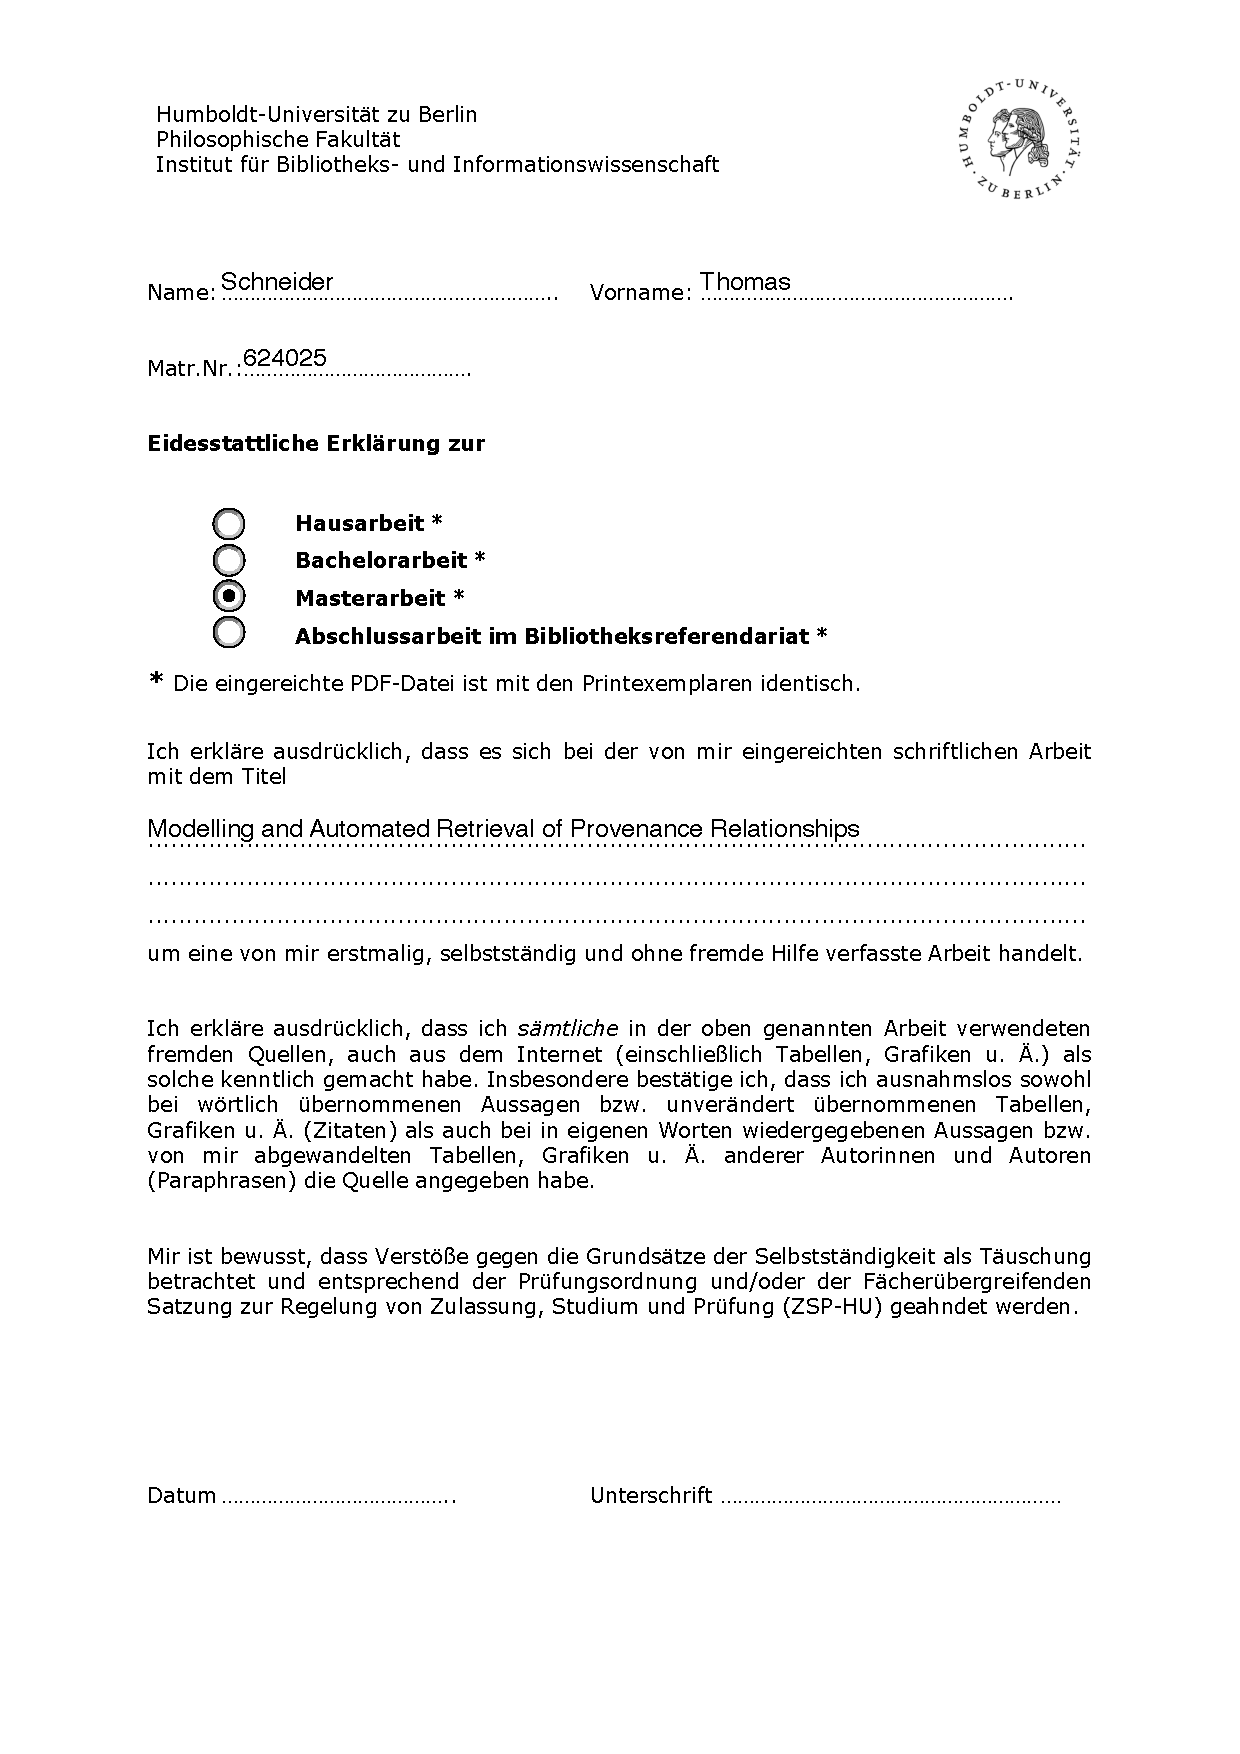
\includepdf{img/Selbststaendigkeitserklaerung_TS_printed.pdf}


\end{document}
